\documentclass[openany]{book}
\author{David Gabriel Corzo Mcmath}
\title{\huge Cálculo Integral \normalsize \\ Notas de clase }
\date{2019-09-20 08:07}
% % % % % % % % % % % % % % % % % % % % % % % % % % % % % % % % % % % % % % % % % % % % % % % % % % %
\usepackage[margin = 1in]{geometry}
\usepackage{graphicx}
\usepackage{fontenc}
\usepackage{pdfpages}
\usepackage[spanish]{babel}
\usepackage{amsmath}
\usepackage{amsthm}
\usepackage[utf8]{inputenc}
\usepackage{enumitem}
\usepackage{mathtools}
\usepackage{import}
\usepackage{xifthen}
\usepackage{pdfpages}
\usepackage{transparent}
\usepackage{color}
\usepackage{fancyhdr}
\usepackage{lipsum}
\usepackage{sectsty}
\usepackage{titlesec}
\usepackage{calc}
\usepackage{lmodern}
\usepackage{xpatch}
\usepackage{blindtext}
\usepackage{bookmark}
\usepackage{fancyhdr}
\usepackage{xcolor}
\usepackage{tikz}
\usepackage{blindtext}
%%%%%%%%%%%%%%%%%%%%%%%%%%%%%%%%%%%%%%%%%%%%%%%%%%%%%%%%%%%%%%%%%%%%%%%%%%%%%%%%%%%%%%%%%%%%%%%%
% Clear the header and footer
\fancyhead{}
\fancyfoot{}
% Set the right side of the footer to be the page number
{\fontfamily{mc}\selectfont
\fancyfoot[L]{\thepage}
\fancypagestyle{plain}{
    \renewcommand{\headrulewidth}{0pt}
    \fancyhf{}
    \fancyfoot[L]{\thepage}
}}

% THIS IS TO CENTER AND DEDICATE A CHAPTER NAME AN ENTIRE PAGE
\titleformat{\chapter}[display]
{\vfill\filcenter}
{{%
   \filcenter\fontsize{48pt}{48pt}\usefont{T1}{cm}{m}{n}{\centering\chaptername} 
   \fontsize{80pt}{80pt}\selectfont\thechapter%
 }%
}
{5pt}
{\huge\usefont{T1}{cm}{b}{n}
 \parbox{\textwidth-\widthof{\LARGE\sffamily{\centering\chaptername}}}
}[\vfill\clearpage]

\titlespacing*{\chapter}{0pt}{0pt}{50pt}

% TO SEPATE WHOLE PAGE DEDICATION IN THE TABLE OF CONTENTS
\titleformat{name=\chapter,numberless}[display]
{\filcenter}
{{
 }
}
{5pt}
{\Huge\usefont{T1}{cm}{b}{n}\centering
}







% MAKE THE TITLE OF THE CHAPTER CENTER!!
\makeatletter

\xpatchcmd{\@makeschapterhead}{%
  \Huge \bfseries  #1\par\nobreak%
}{%
  \Huge \bfseries\centering #1\par\nobreak%
}{\typeout{Patched makeschapterhead}}{\typeout{patching of @makeschapterhead failed}}


\xpatchcmd{\@makechapterhead}{%
  \huge\bfseries \@chapapp\space \thechapter
}{%
  \huge\bfseries\centering \@chapapp\space \thechapter
}{\typeout{Patched @makechapterhead}}{\typeout{Patching of @makechapterhead failed}}

\makeatother

% \newcommand*\circled[1]{\tikz[baseline=(char.base)]{
%             \node[shape=circle,fill=gray!50,inner sep=2pt] (char) {#1};}}

% % header style
% \pagestyle{fancy}
% \fancyhf{}
% \fancyhead[EL]{\nouppercase\leftmark}
% \fancyhead[OR]{\nouppercase\rightmark}
% \fancyfoot[C]{\circled{\thepage}}
\newcommand*\circled[1]{\tikz[baseline=(char.base)]{
            \node[shape=circle,fill=gray!50,inner sep=2pt] (char) {#1};}}

% header style
\pagestyle{fancy}
\fancyhf{}
\fancyhead[EL]{\nouppercase\leftmark}
\fancyhead[OR]{\nouppercase\rightmark}
\fancyfoot[C]{\circled{\thepage}}

\fancypagestyle{plain}{%
  \fancyhf{}
  \fancyfoot[C]{\circled{\thepage}}
  \renewcommand{\headrulewidth}{0pt}
}



% % % % % % % % % % % % % % % % % % % % % % % % % % % % % % % % % % % % % % % % % % % % % % % % % % %
\begin{document}
\maketitle
\tableofcontents


\part{Material de clase, Notas}

\chapter{Antiderivadas, integrales indefinidas, notación de integral, reglas básicas de integración, integrales definidas, Teorema fundamental del cálculo}
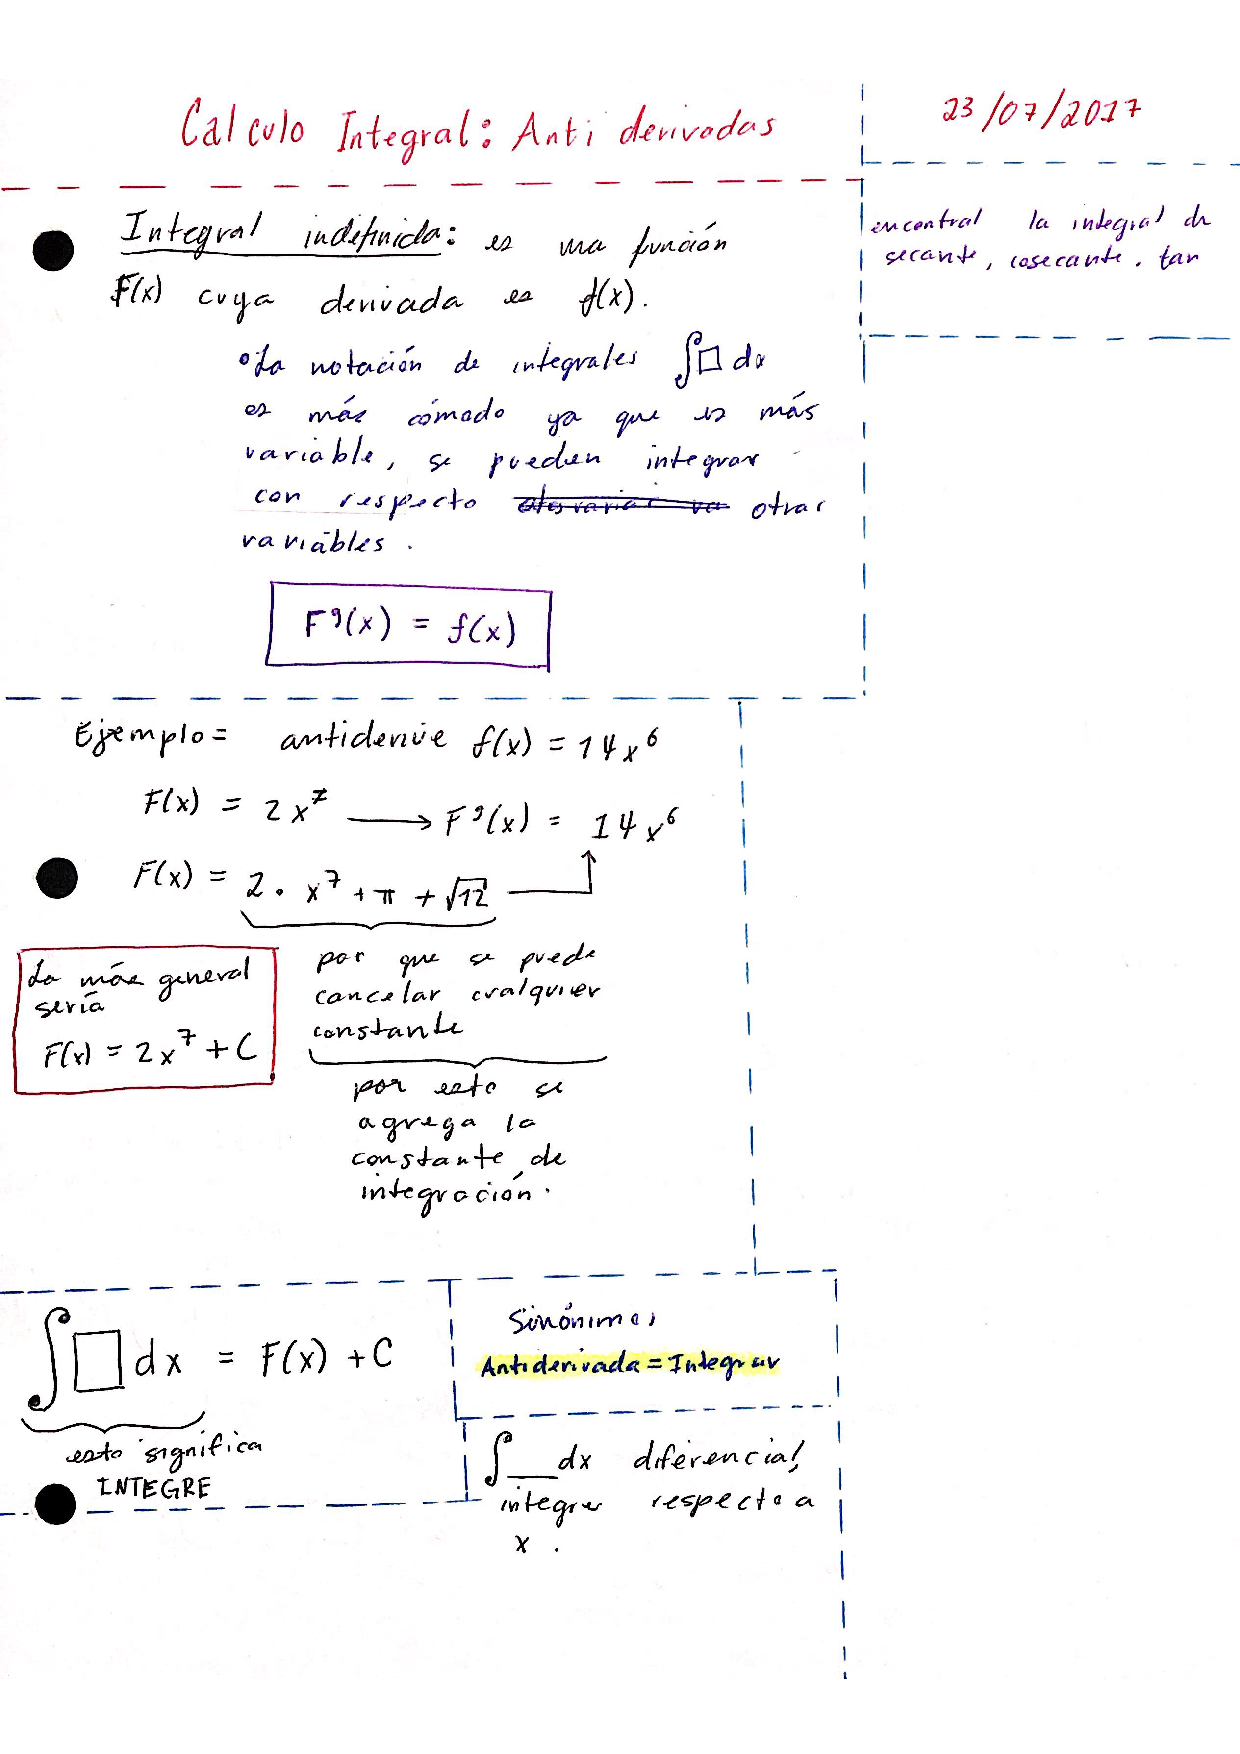
\includepdf[pages=-,pagecommand={\thispagestyle{plain}}]{pdf/MC_01-2019-07-23.pdf}
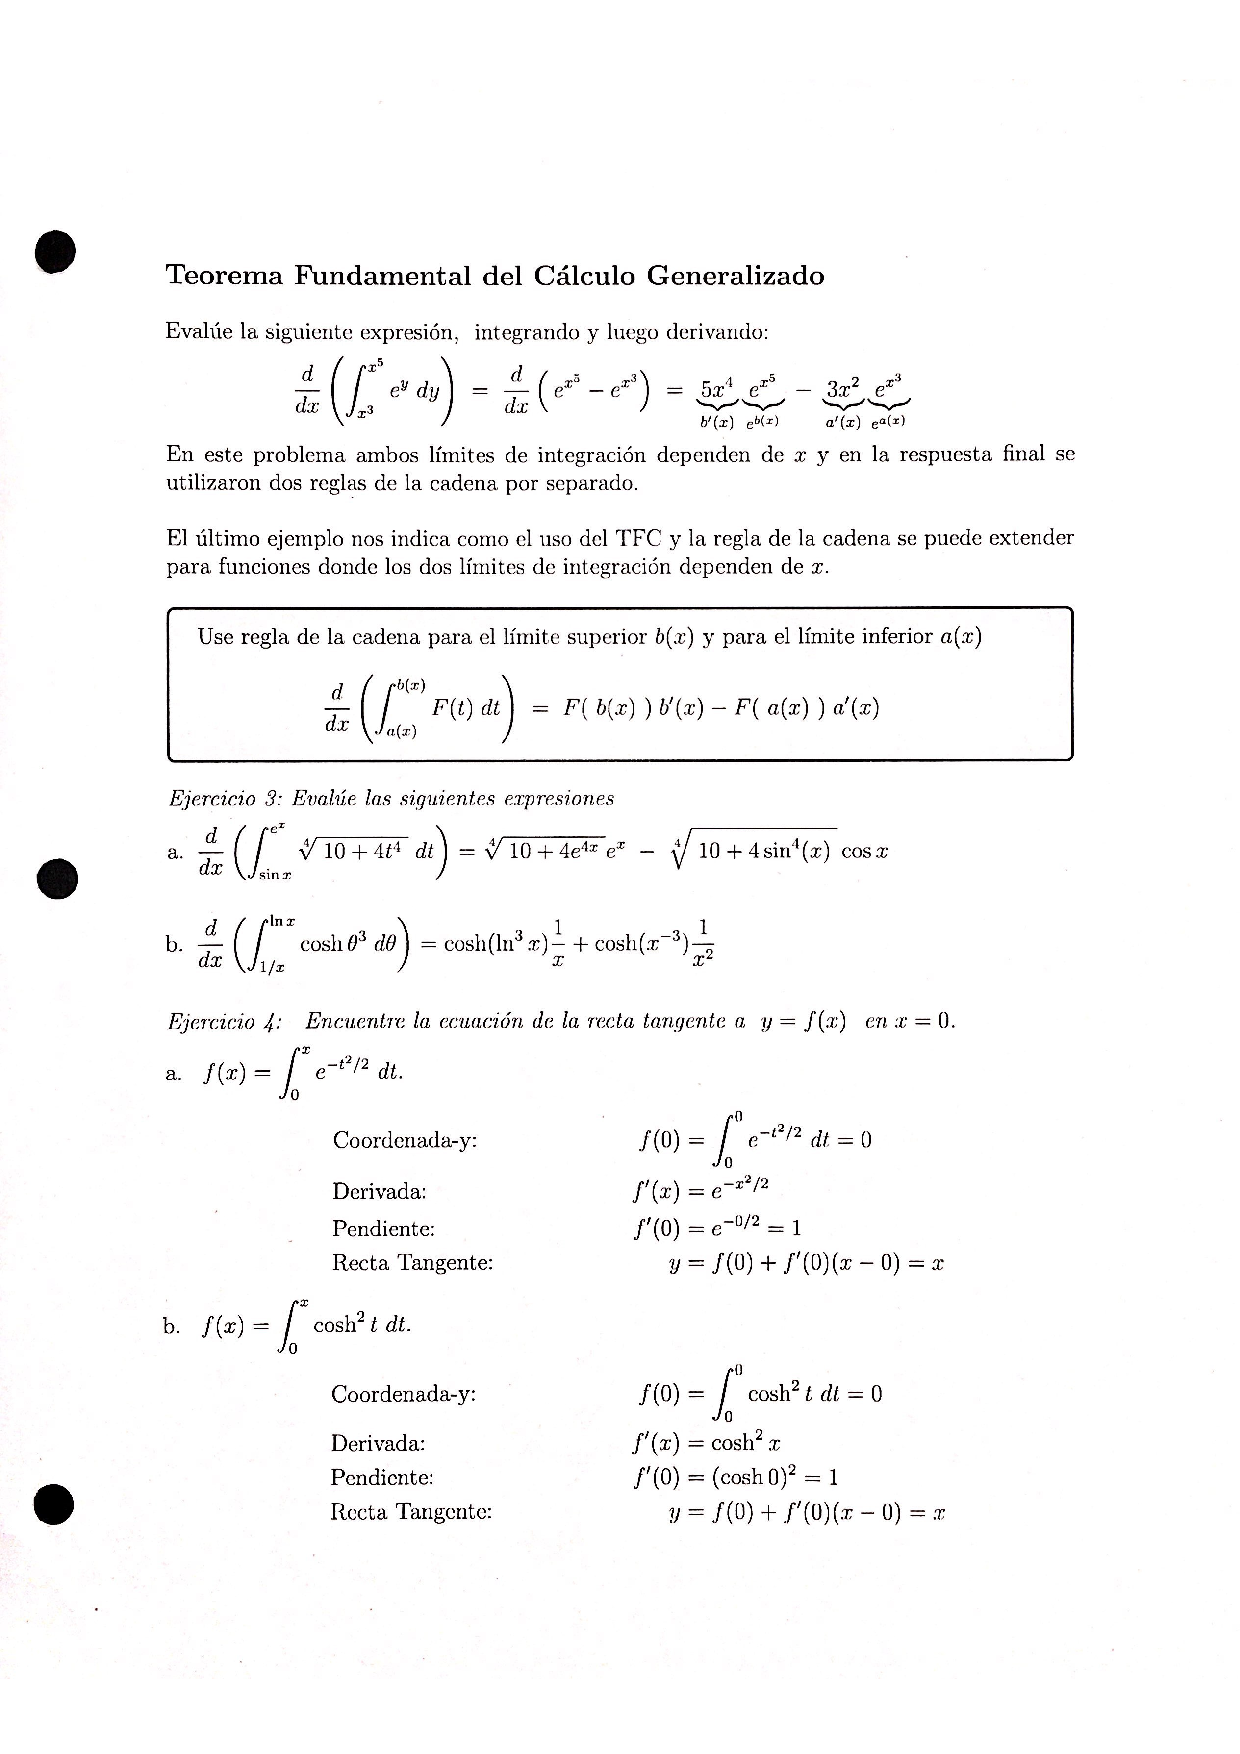
\includepdf[pages=-,pagecommand={\thispagestyle{plain}}]{pdf/DA_3.pdf}


\chapter{Área, desplazamiento y propiedades, sobre vuelo acerca de la regla de la integral definida (inversión de límites con signo negativo), propiedades de integrales definidas, fórmula de área \& fórmula de desplazamiento.}
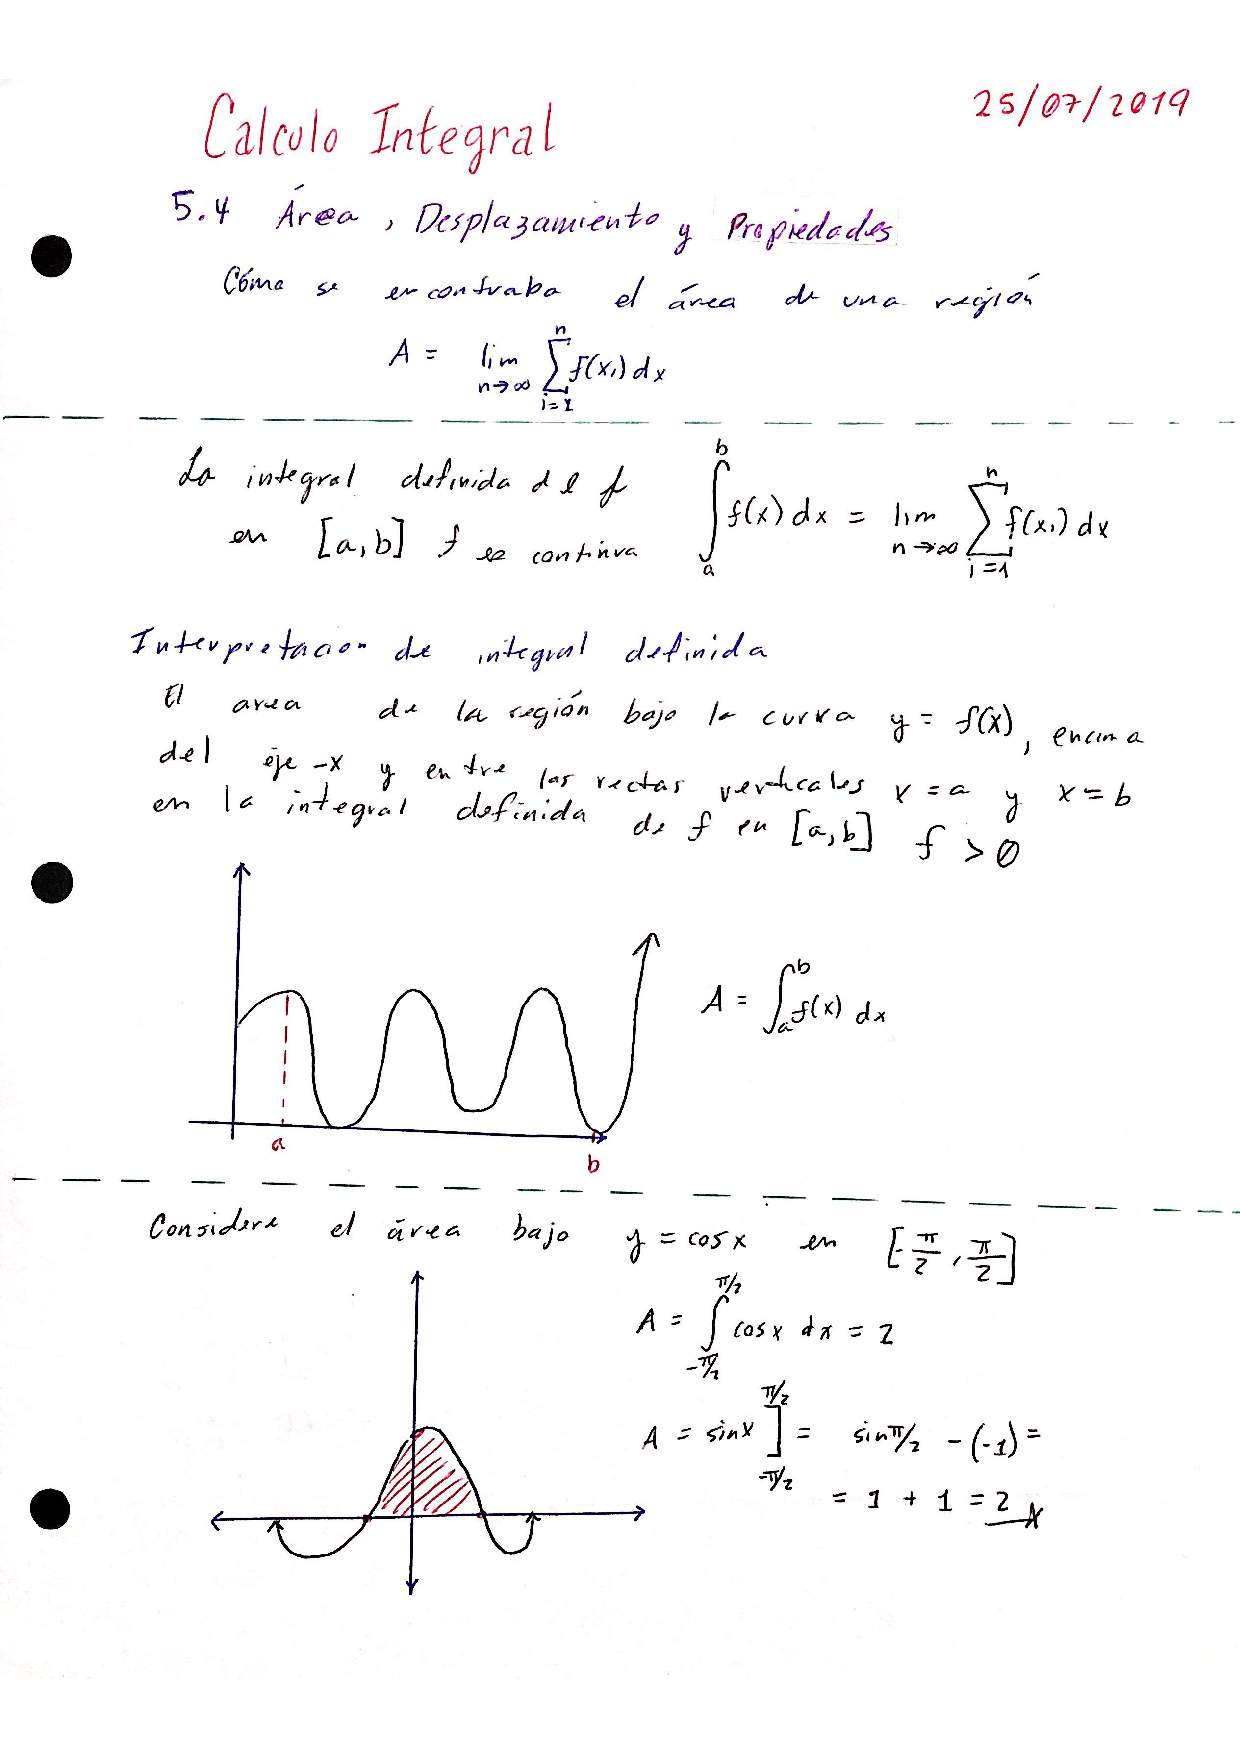
\includepdf[pages=-,pagecommand={\thispagestyle{plain}}]{pdf/MC_02-2019-07-25.pdf}


\chapter{Desplazamiento \& Distancias, presencia de las integrales en la economía, aceleración, velocidad, desplazamiento a partir de una función integrable; propiedad de funciones pares e impares.}
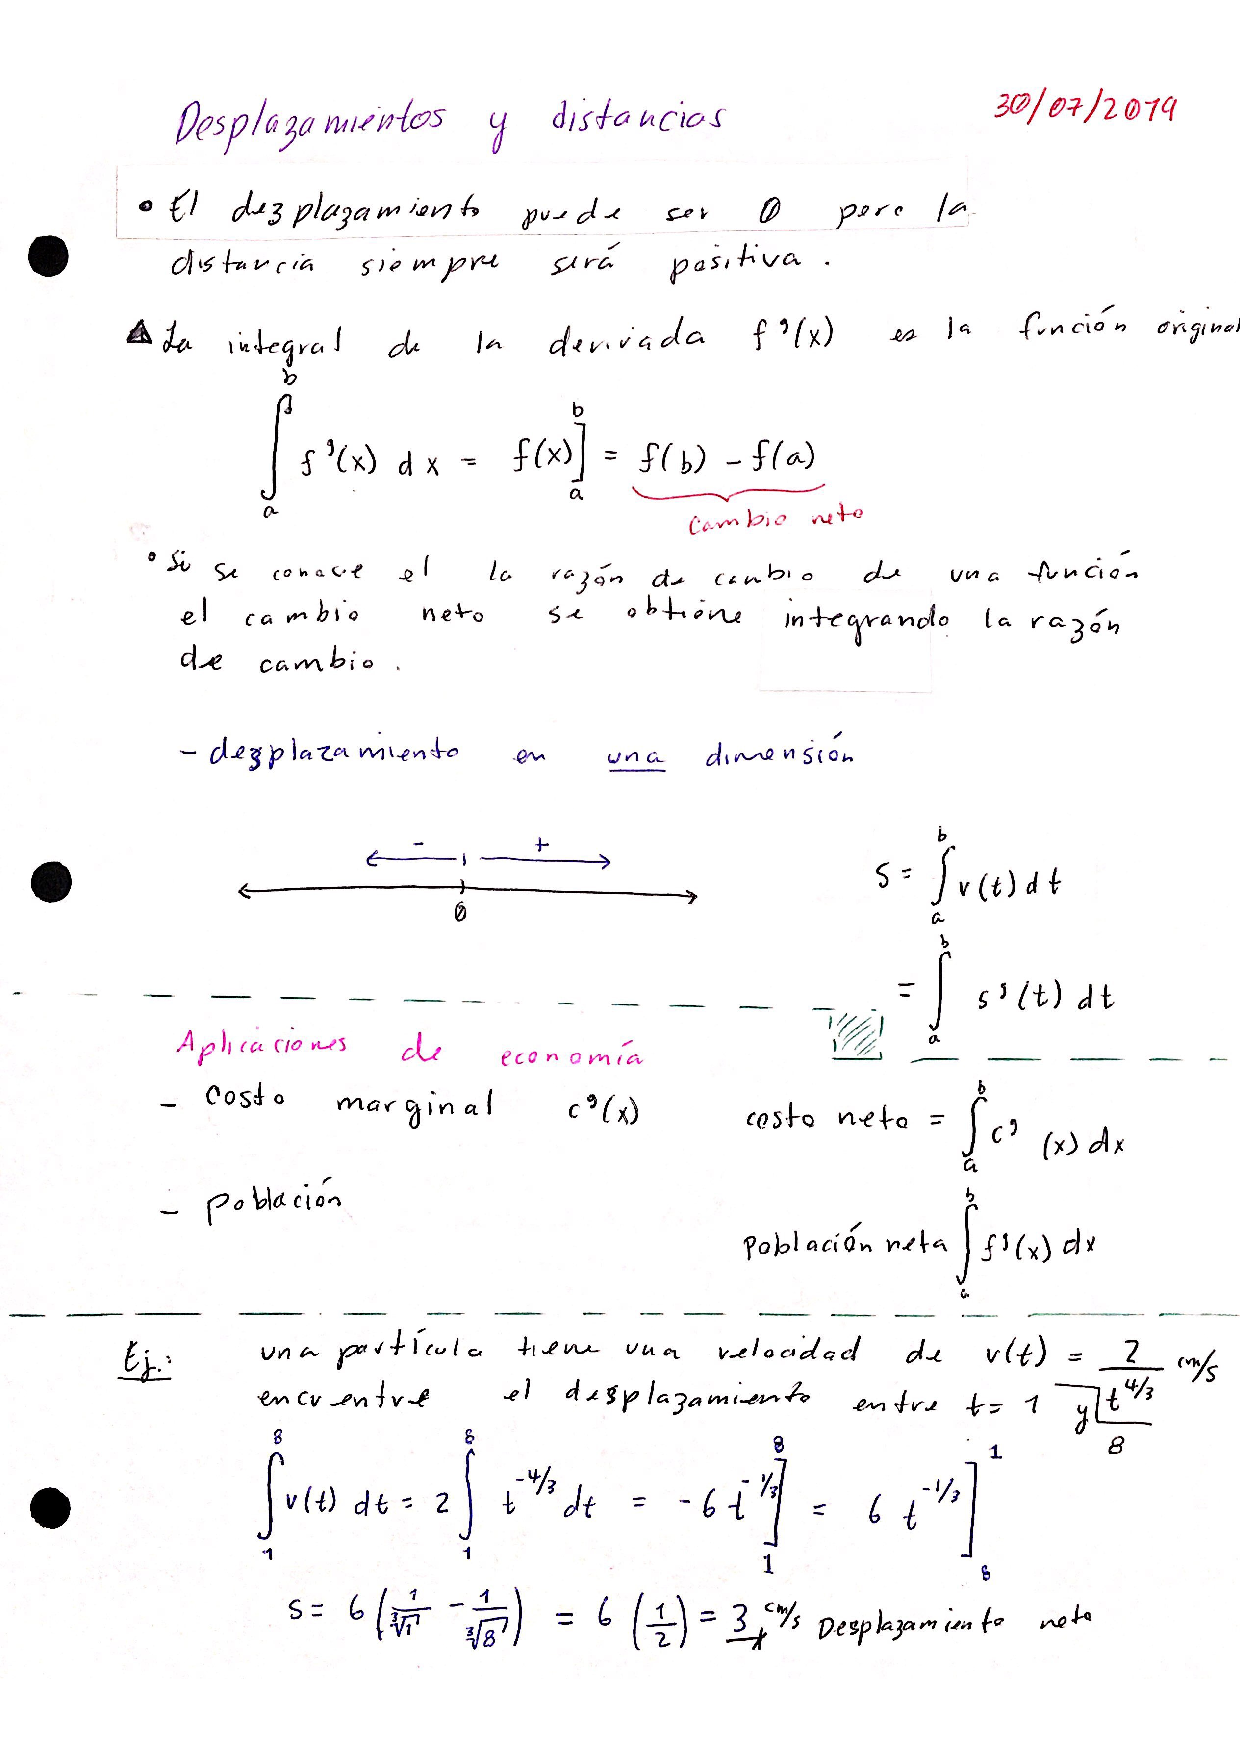
\includepdf[pages=-,pagecommand={\thispagestyle{plain}}]{pdf/MC_03-2019-07-30.pdf}


\chapter{Teorema fundamental del cálculo parte I \& parte II, ¿Cómo utilizo este teorema para derivar integrales con límites?}
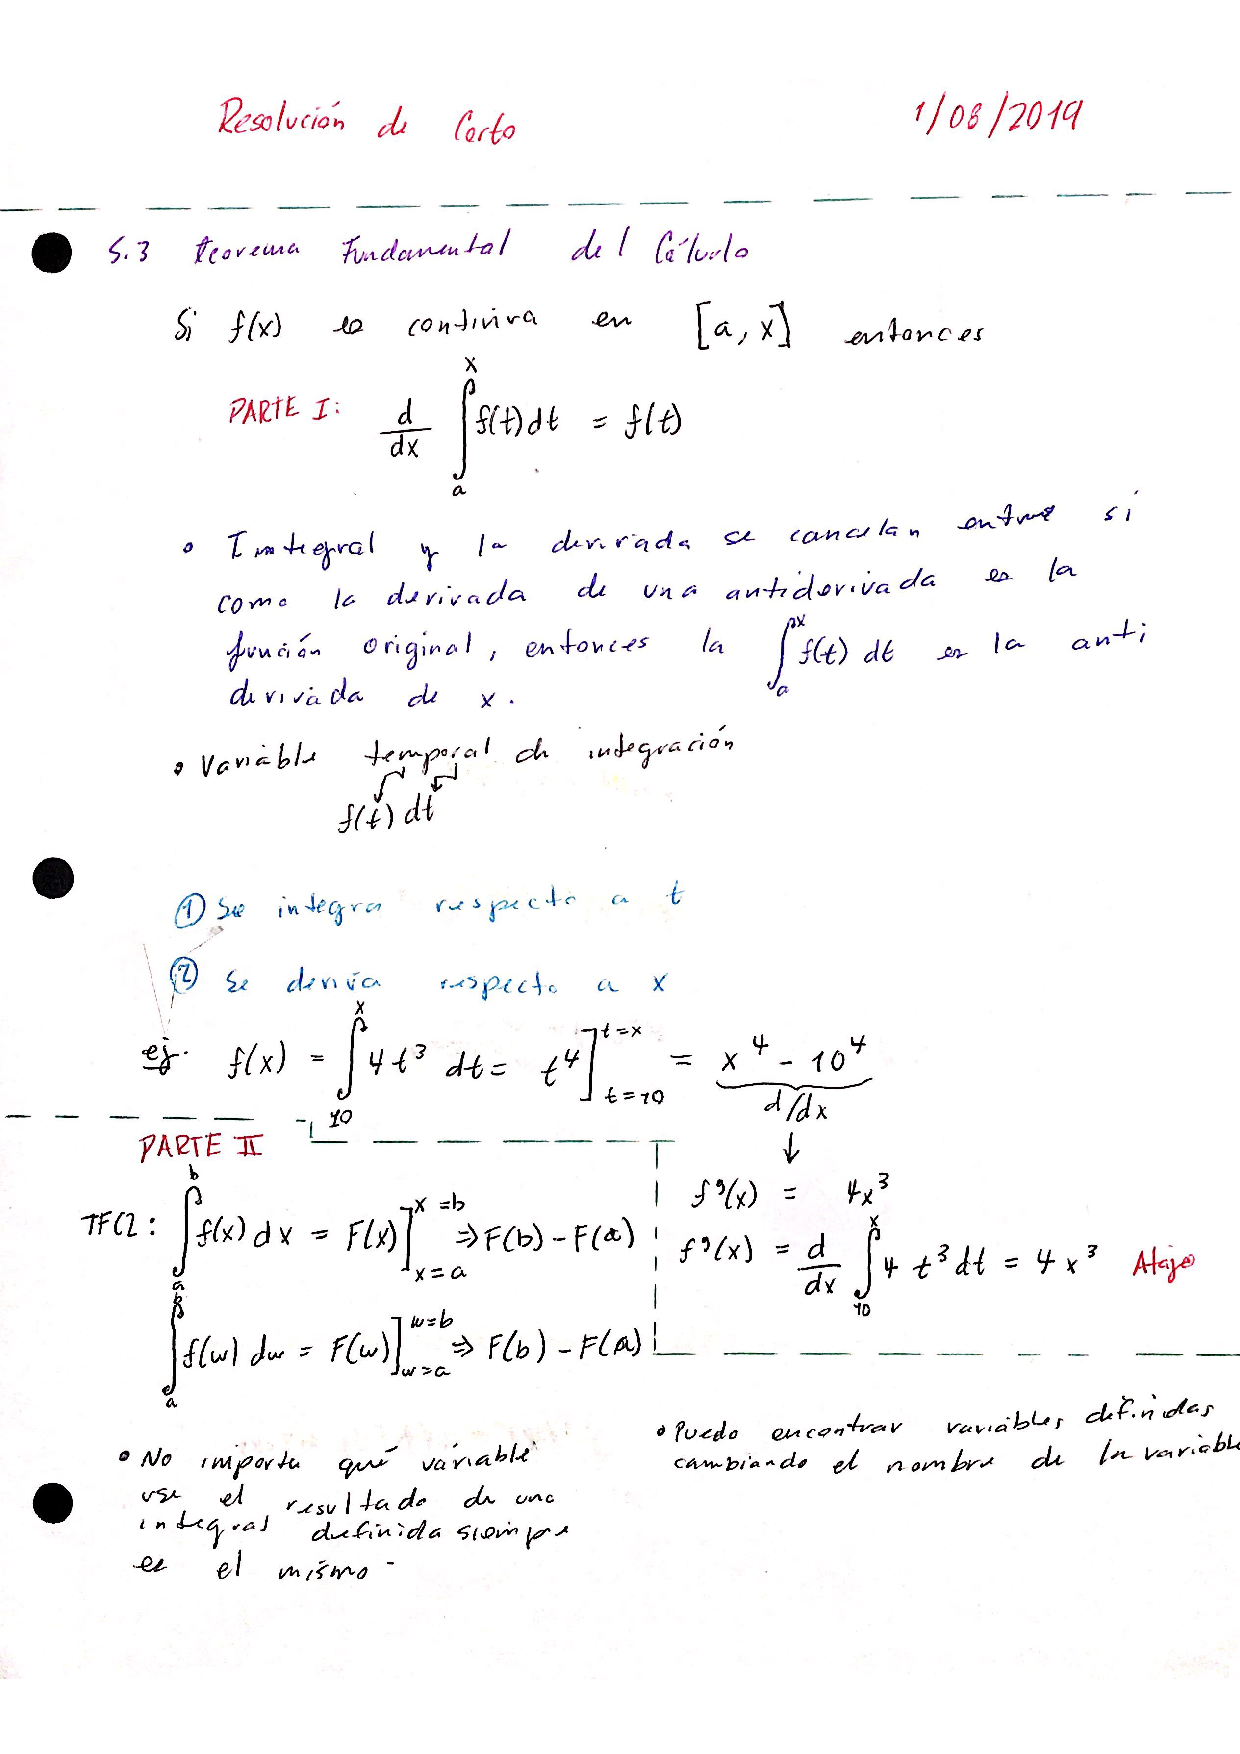
\includepdf[pages=-,pagecommand={\thispagestyle{plain}}]{pdf/MC_04-2019-08-01.pdf}


\chapter{Regla de la sustitución, equivalente a la regla de la cadena en derivadas solo que con integración}
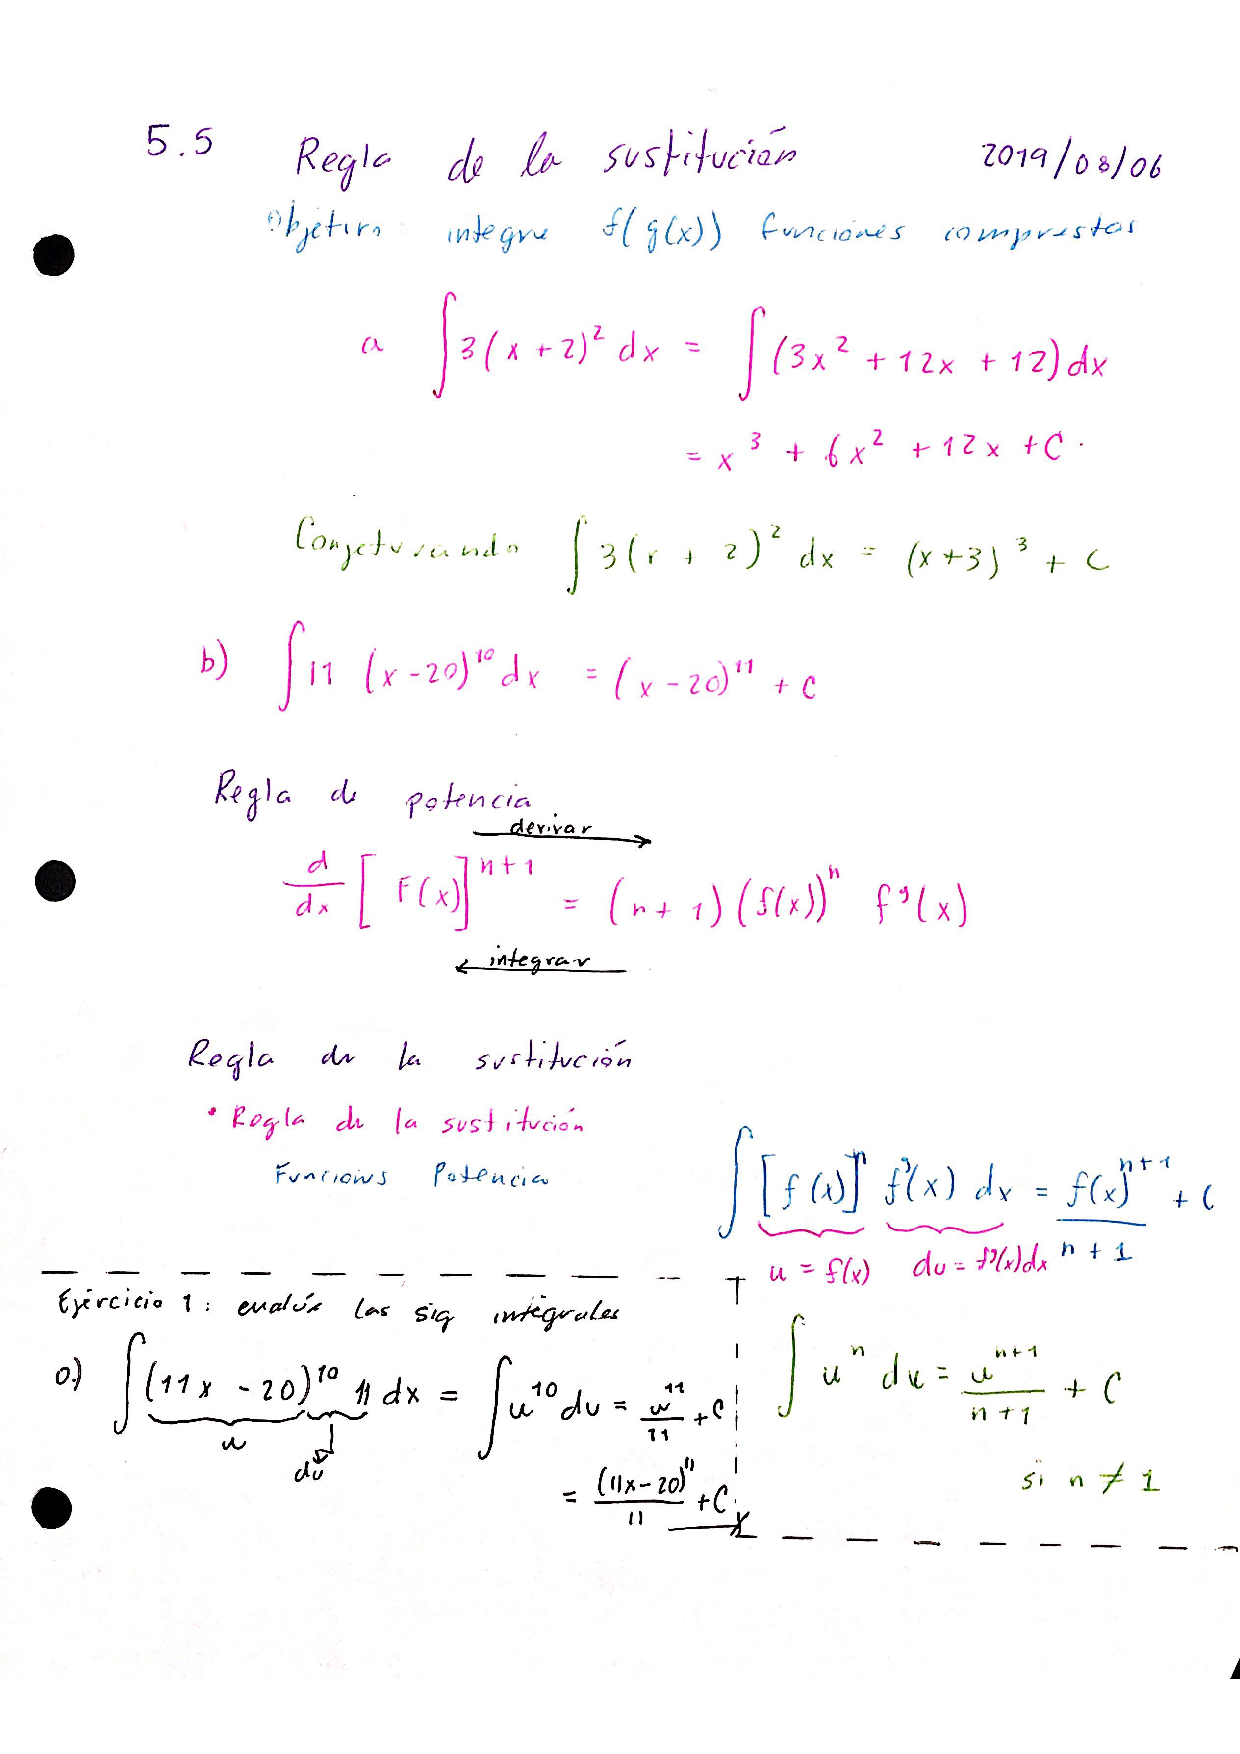
\includepdf[pages=-,pagecommand={\thispagestyle{plain}}]{pdf/MC_05-2019-08-06.pdf}


\chapter{Integración por partes (IPP), ILATE ó LIPET, IPP para definidas}
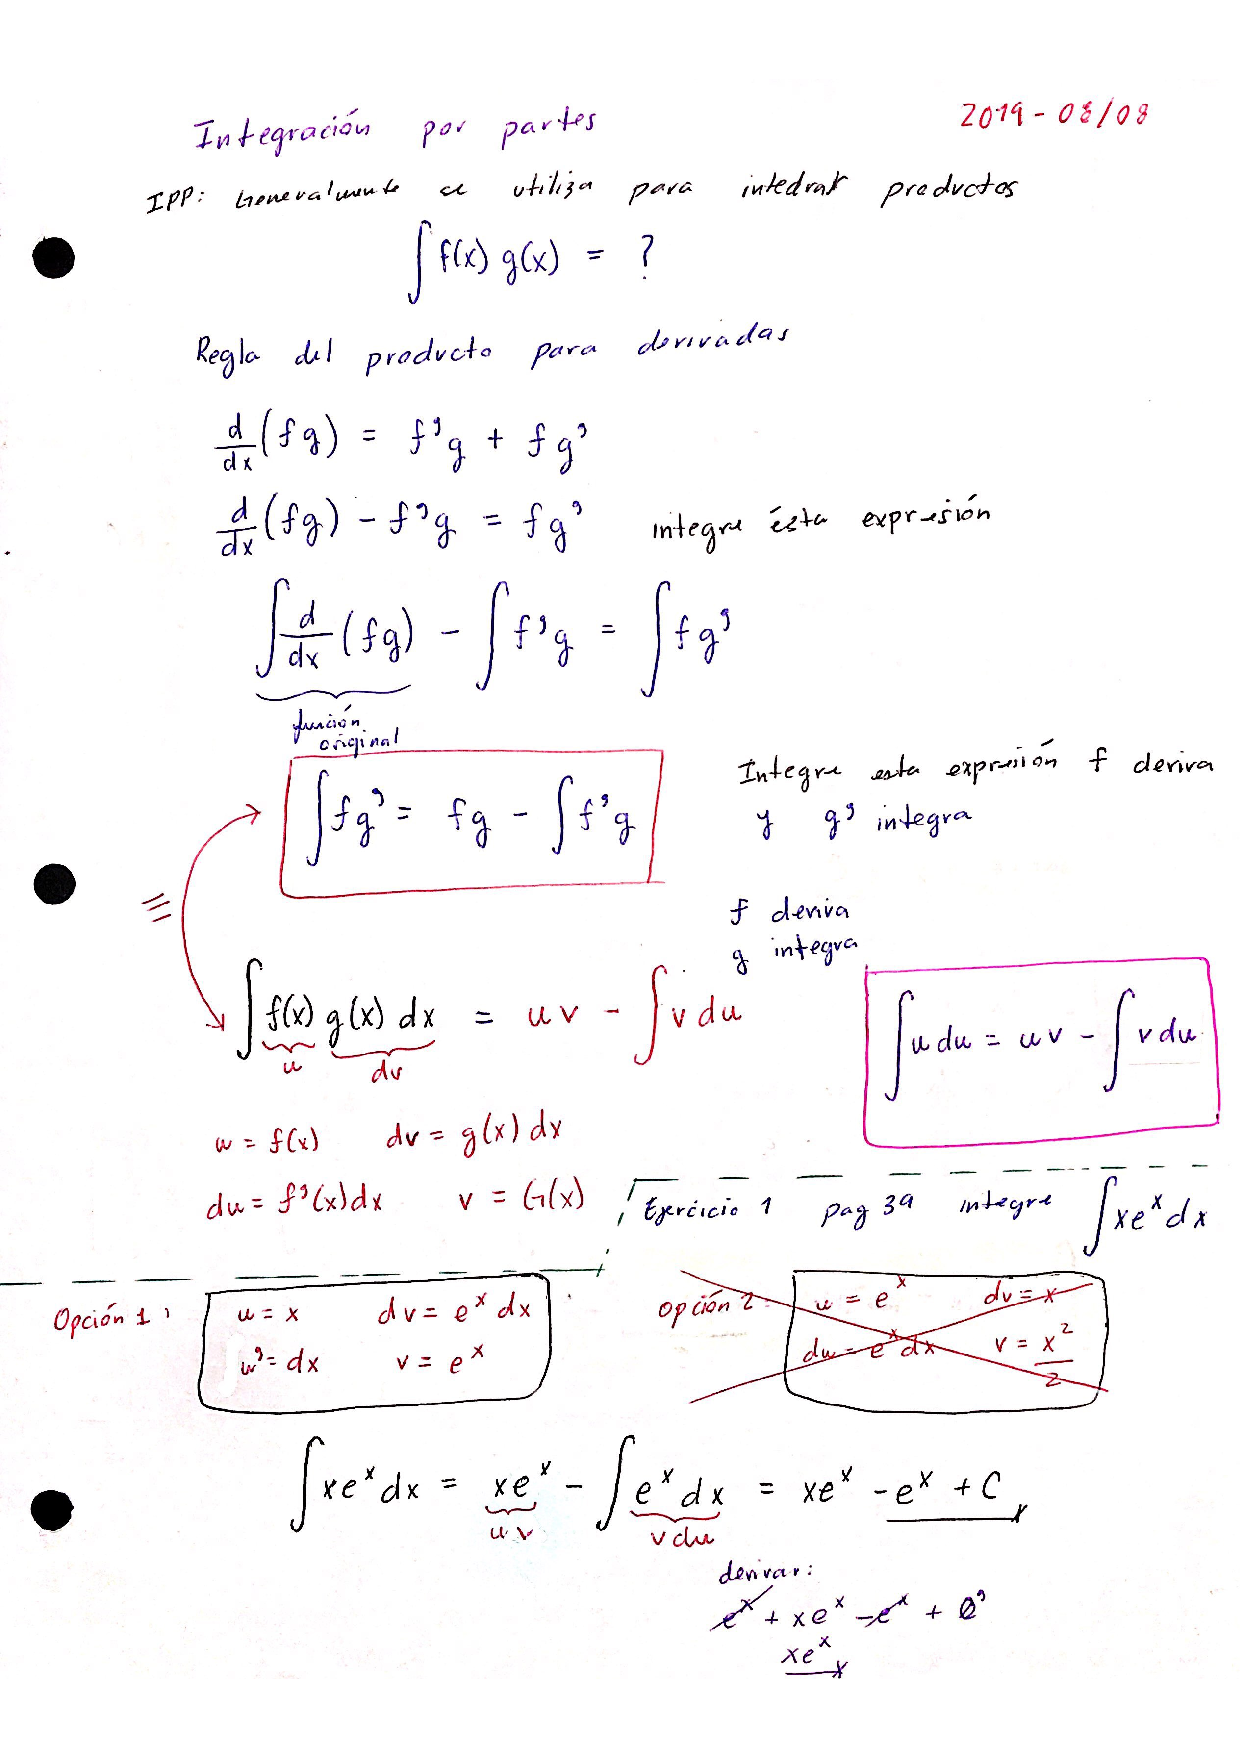
\includepdf[pages=-,pagecommand={\thispagestyle{plain}}]{pdf/MC_06-2019-08-08.pdf}


\chapter{Integrales trigonométricas, explorar las formas y los casos especiales}
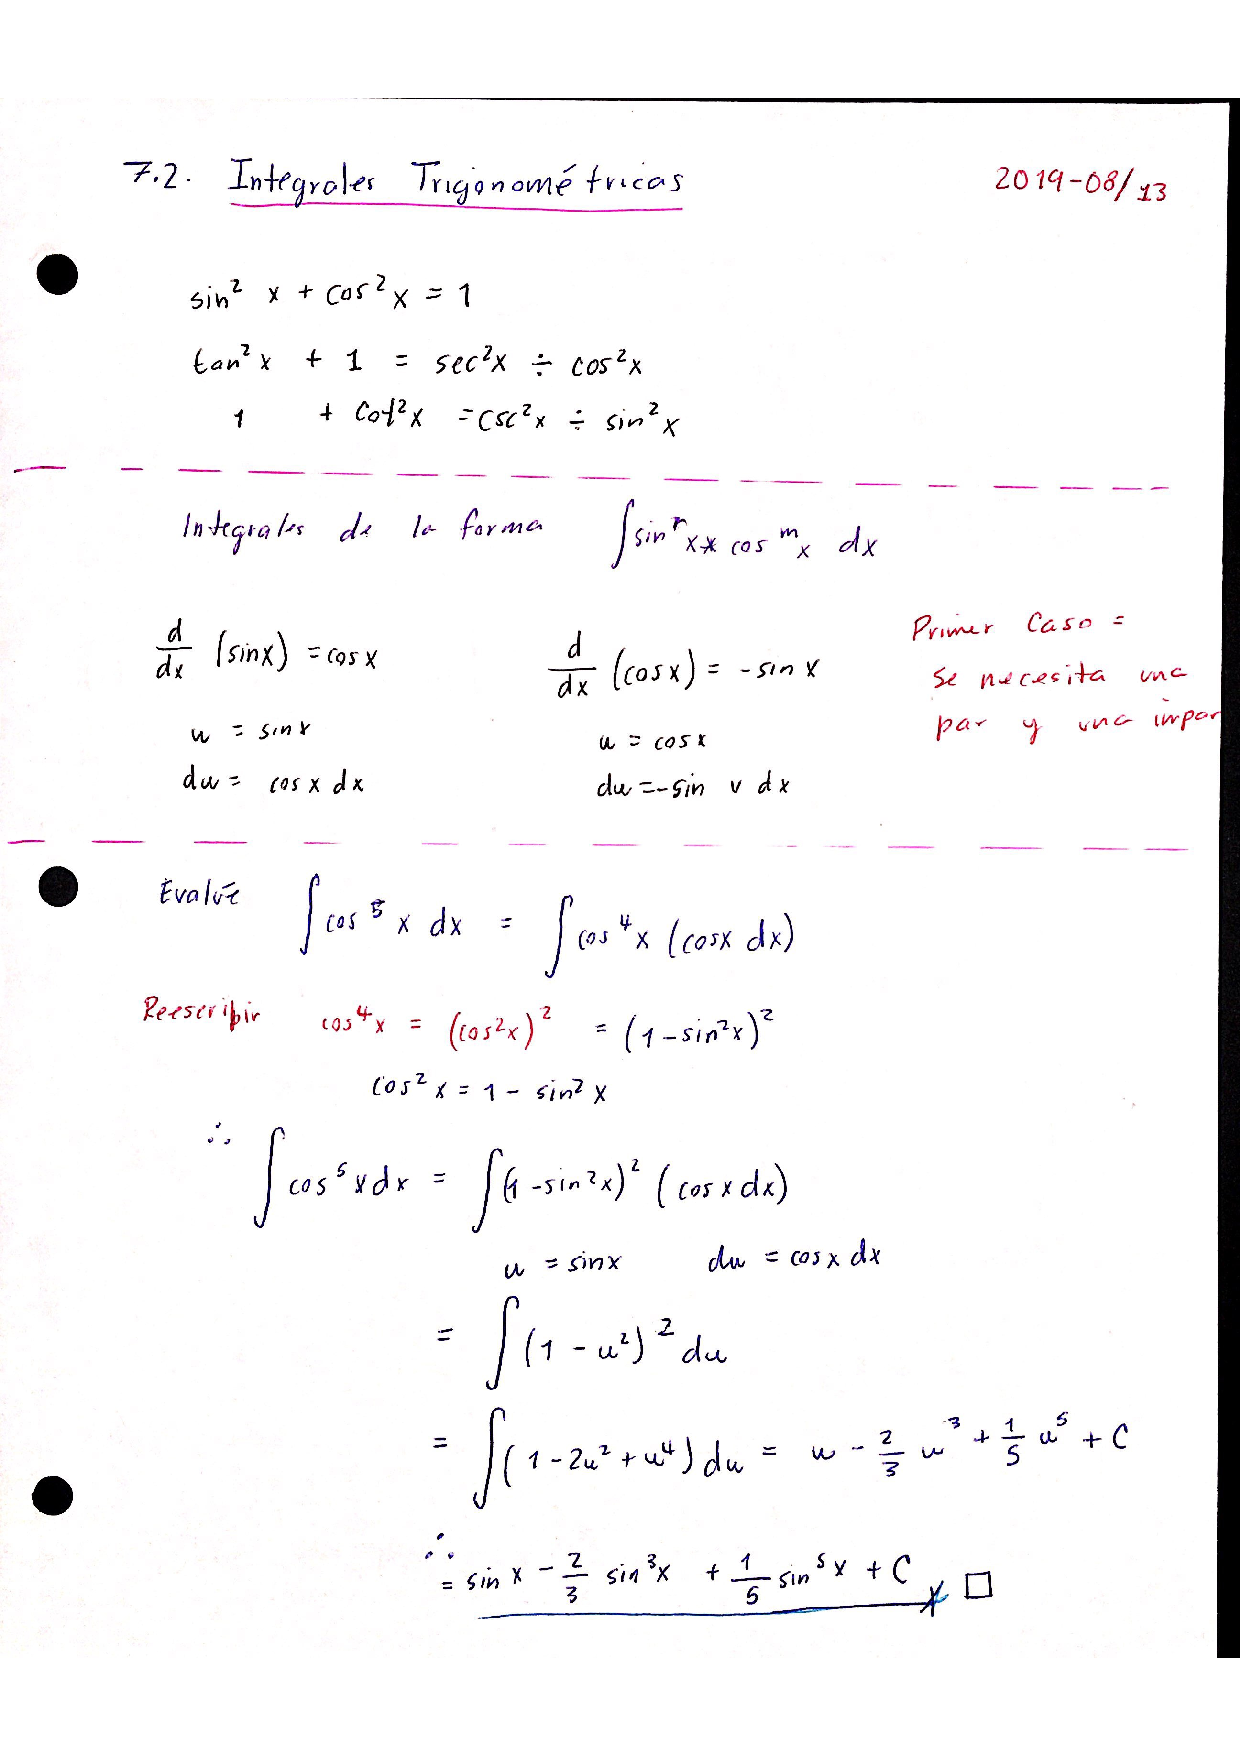
\includepdf[pages=-,pagecommand={\thispagestyle{plain}}]{pdf/MC_07-2019-08-13.pdf}


\chapter{Continuación de Integración trigonométricas, curioso: Área de un circulo unitario, introducción a sustitución trigonométrica}
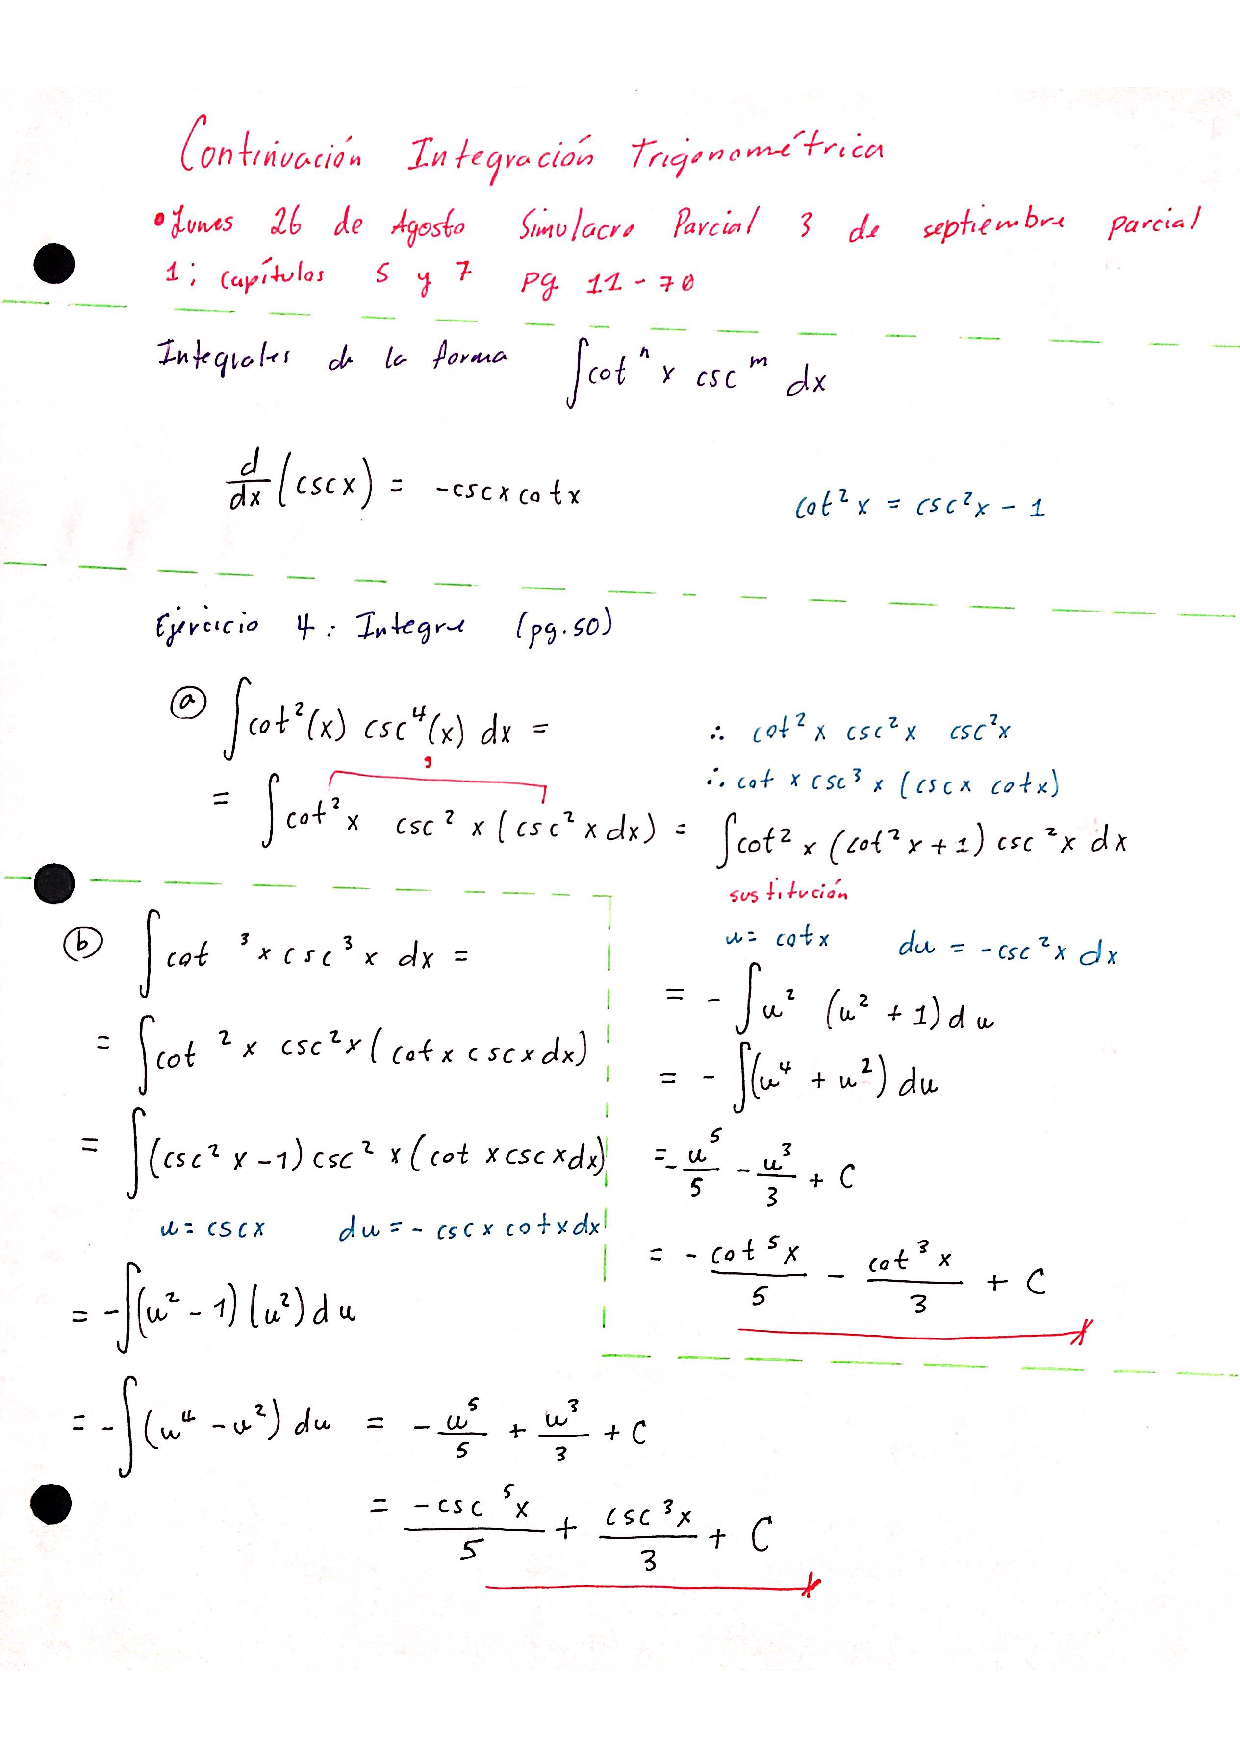
\includepdf[pages=-,pagecommand={\thispagestyle{plain}}]{pdf/MC_08-2019-08-20.pdf}


\chapter{Integración por sustitución trigonométrica}
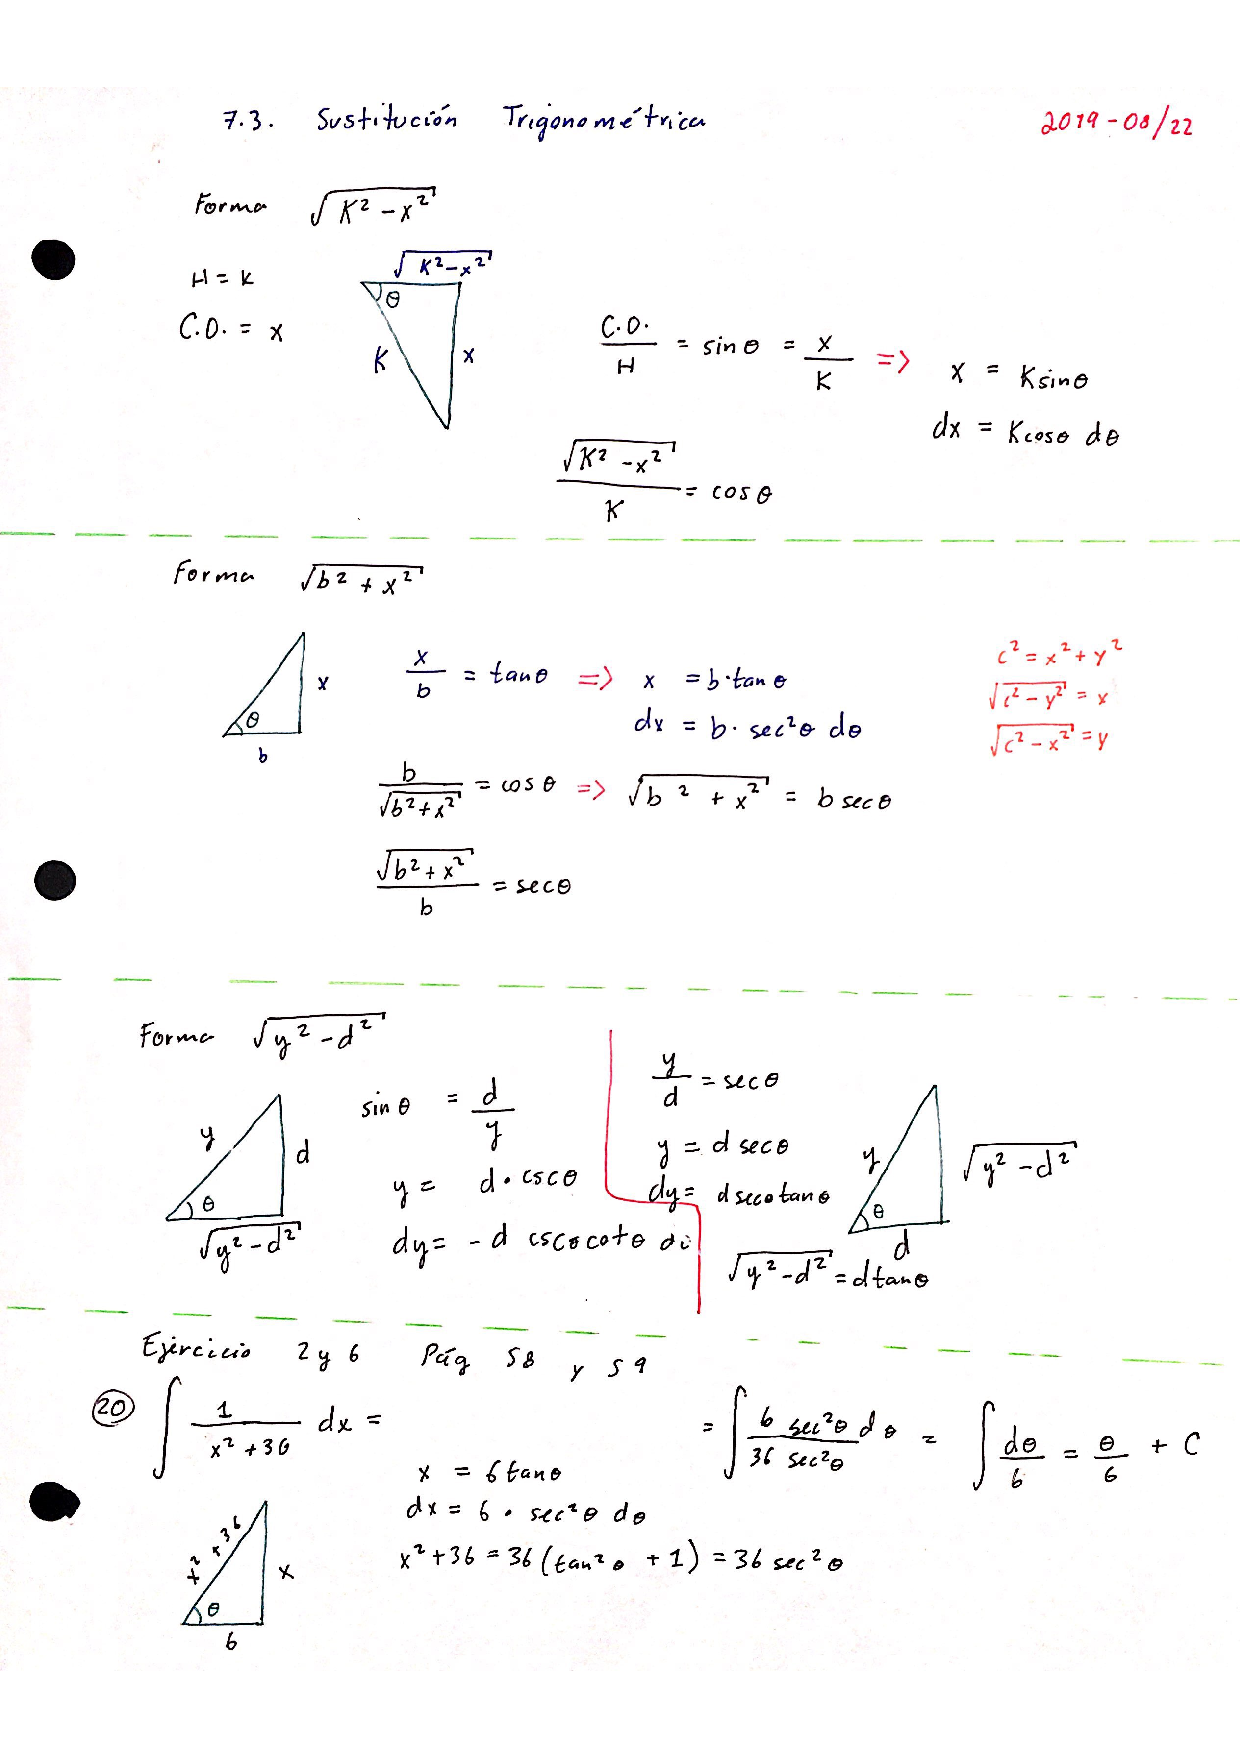
\includepdf[pages=-,pagecommand={\thispagestyle{plain}}]{pdf/MC_09-2019-08-22.pdf}


\chapter{Repaso de sustitución trigonométrica} %Continuación integración por sustitución trigonométrica
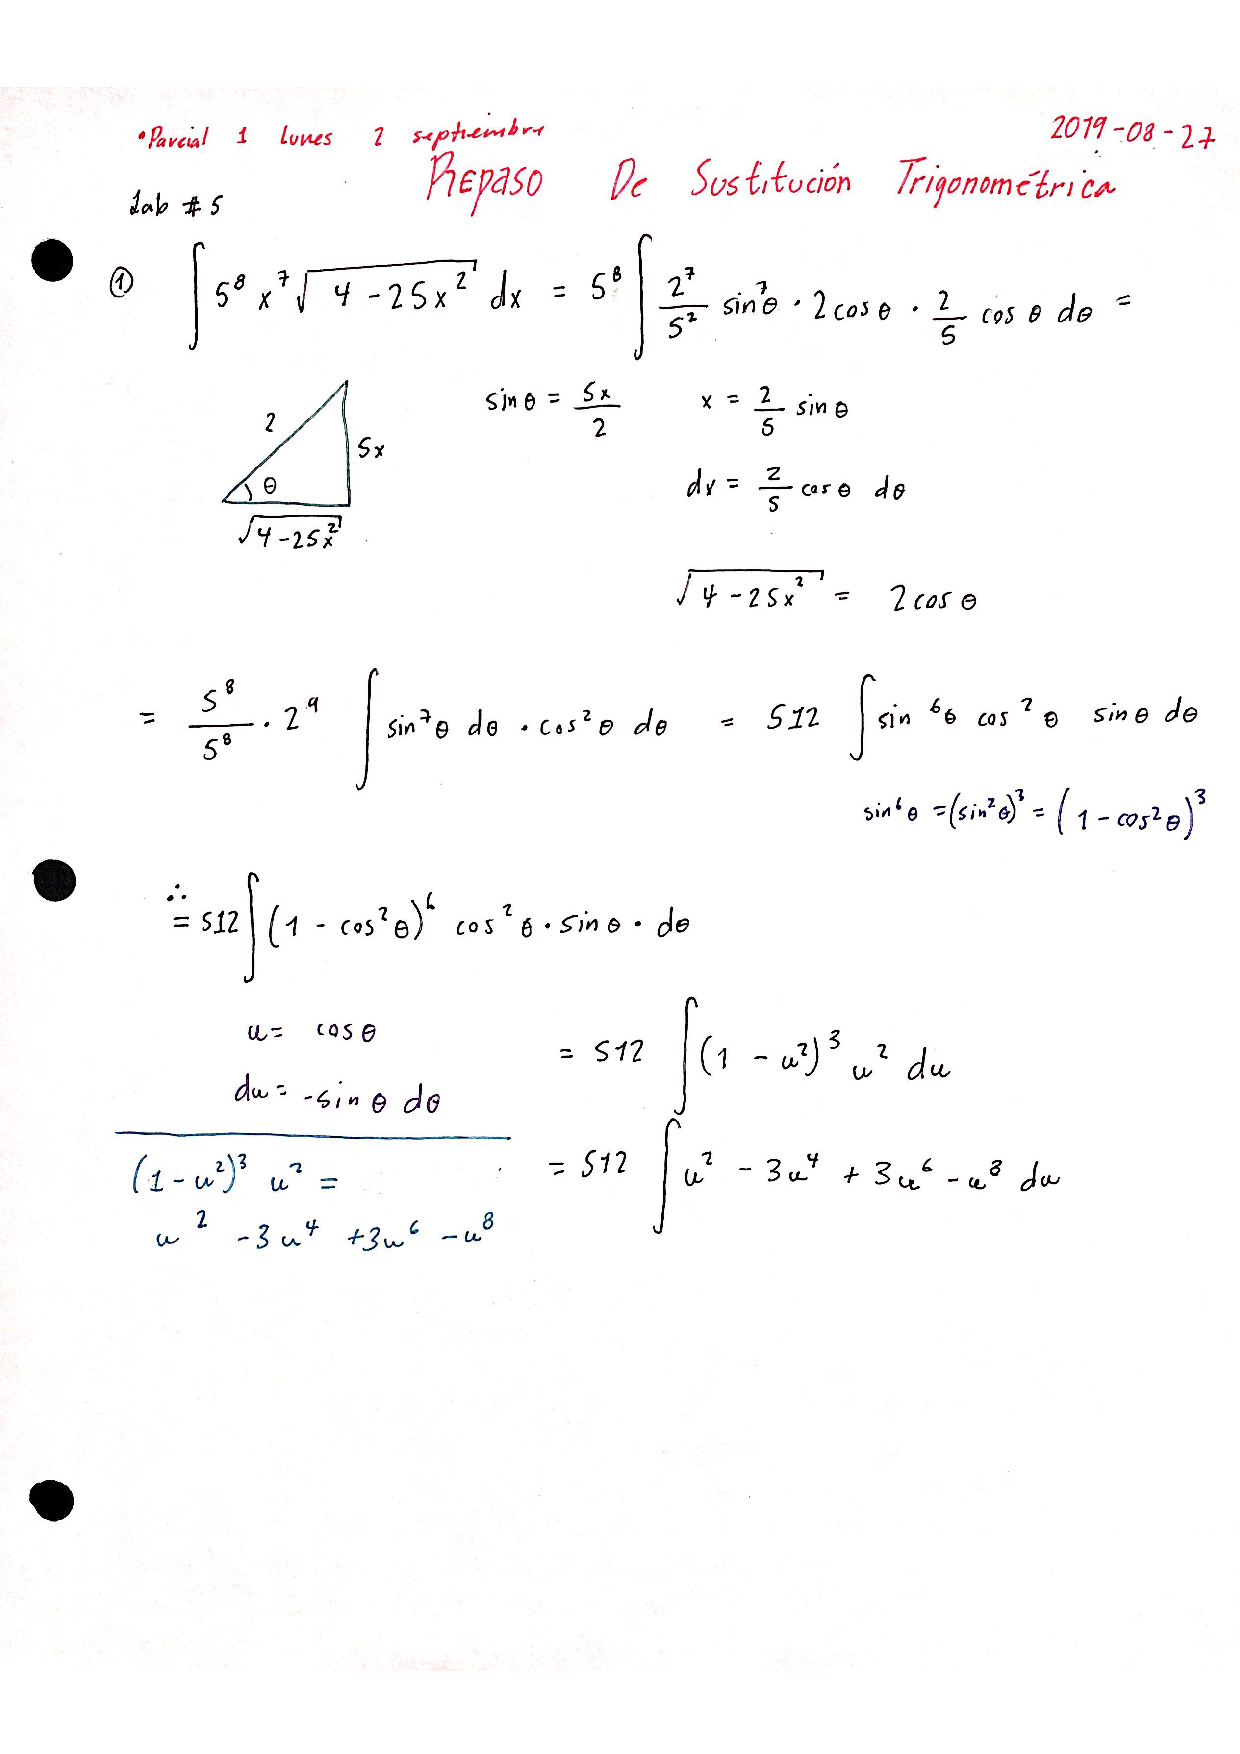
\includepdf[pages=-,pagecommand={\thispagestyle{plain}}]{pdf/MC_10-2019-08-27.pdf}


\chapter{Repaso del parcial simulacro}
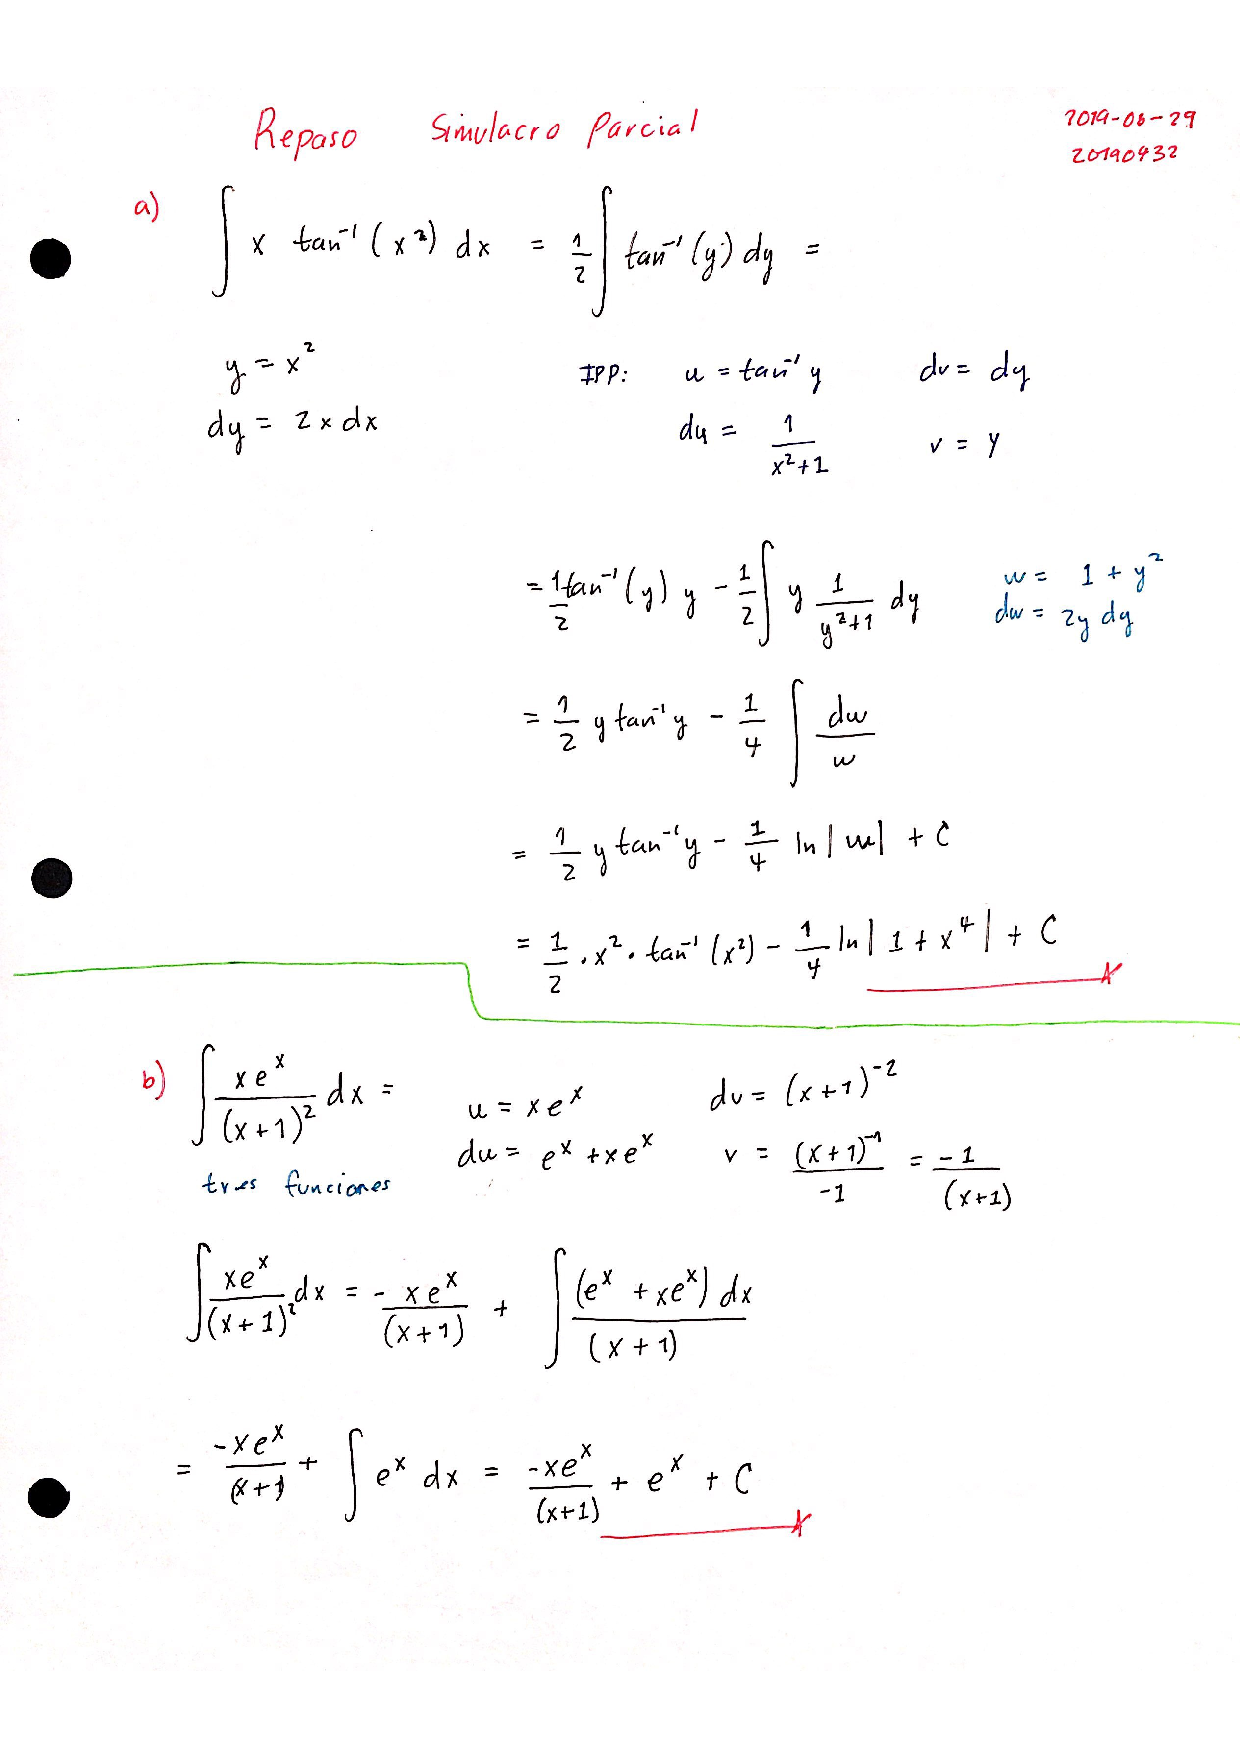
\includepdf[pages=-,pagecommand={\thispagestyle{plain}}]{pdf/MC_11-2019-08-29.pdf}


\chapter{Integrales impropias, tipo uno \& tipo dos}
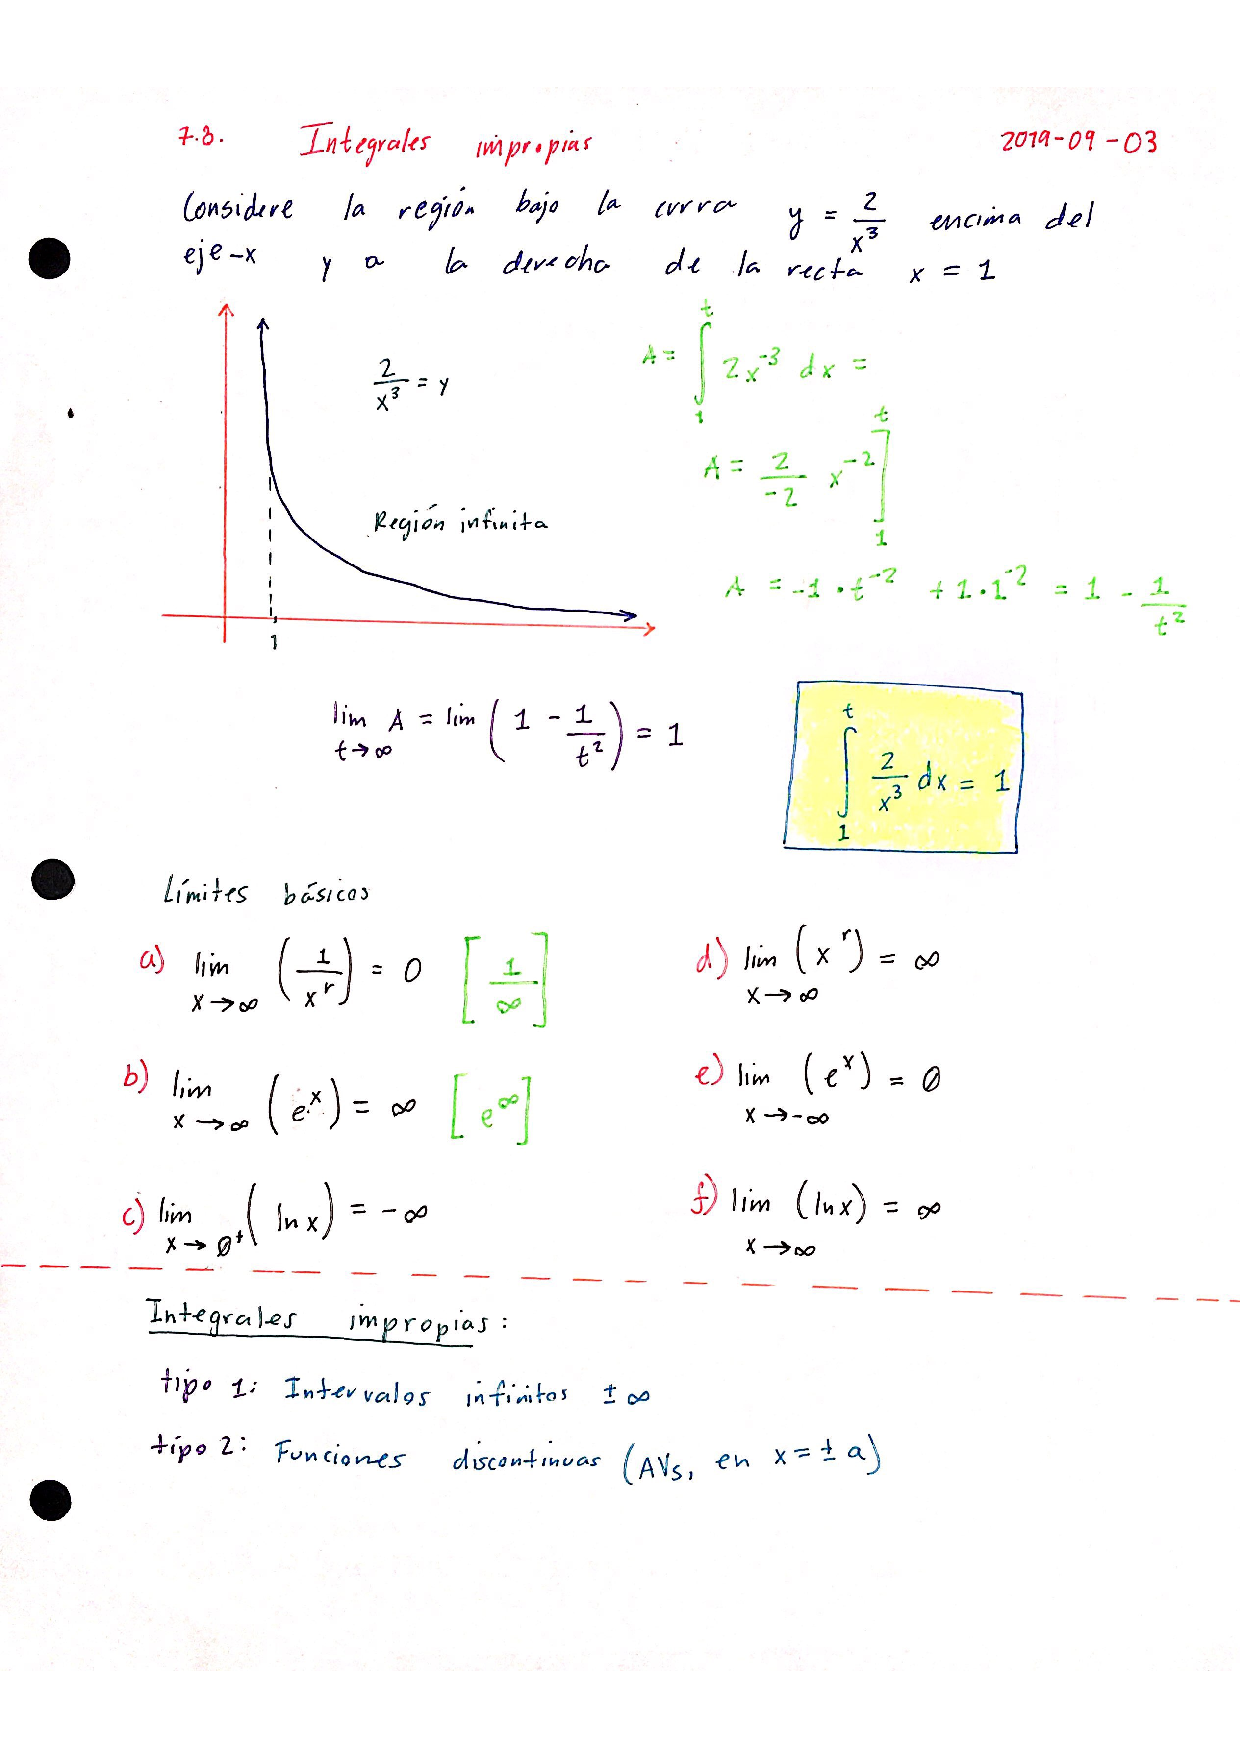
\includepdf[pages=-,pagecommand={\thispagestyle{plain}}]{pdf/MC_12-2019-09-03.pdf}


\chapter{\textbf{Área entre curvas}, pasos para sacar área entre curvas irregulares}
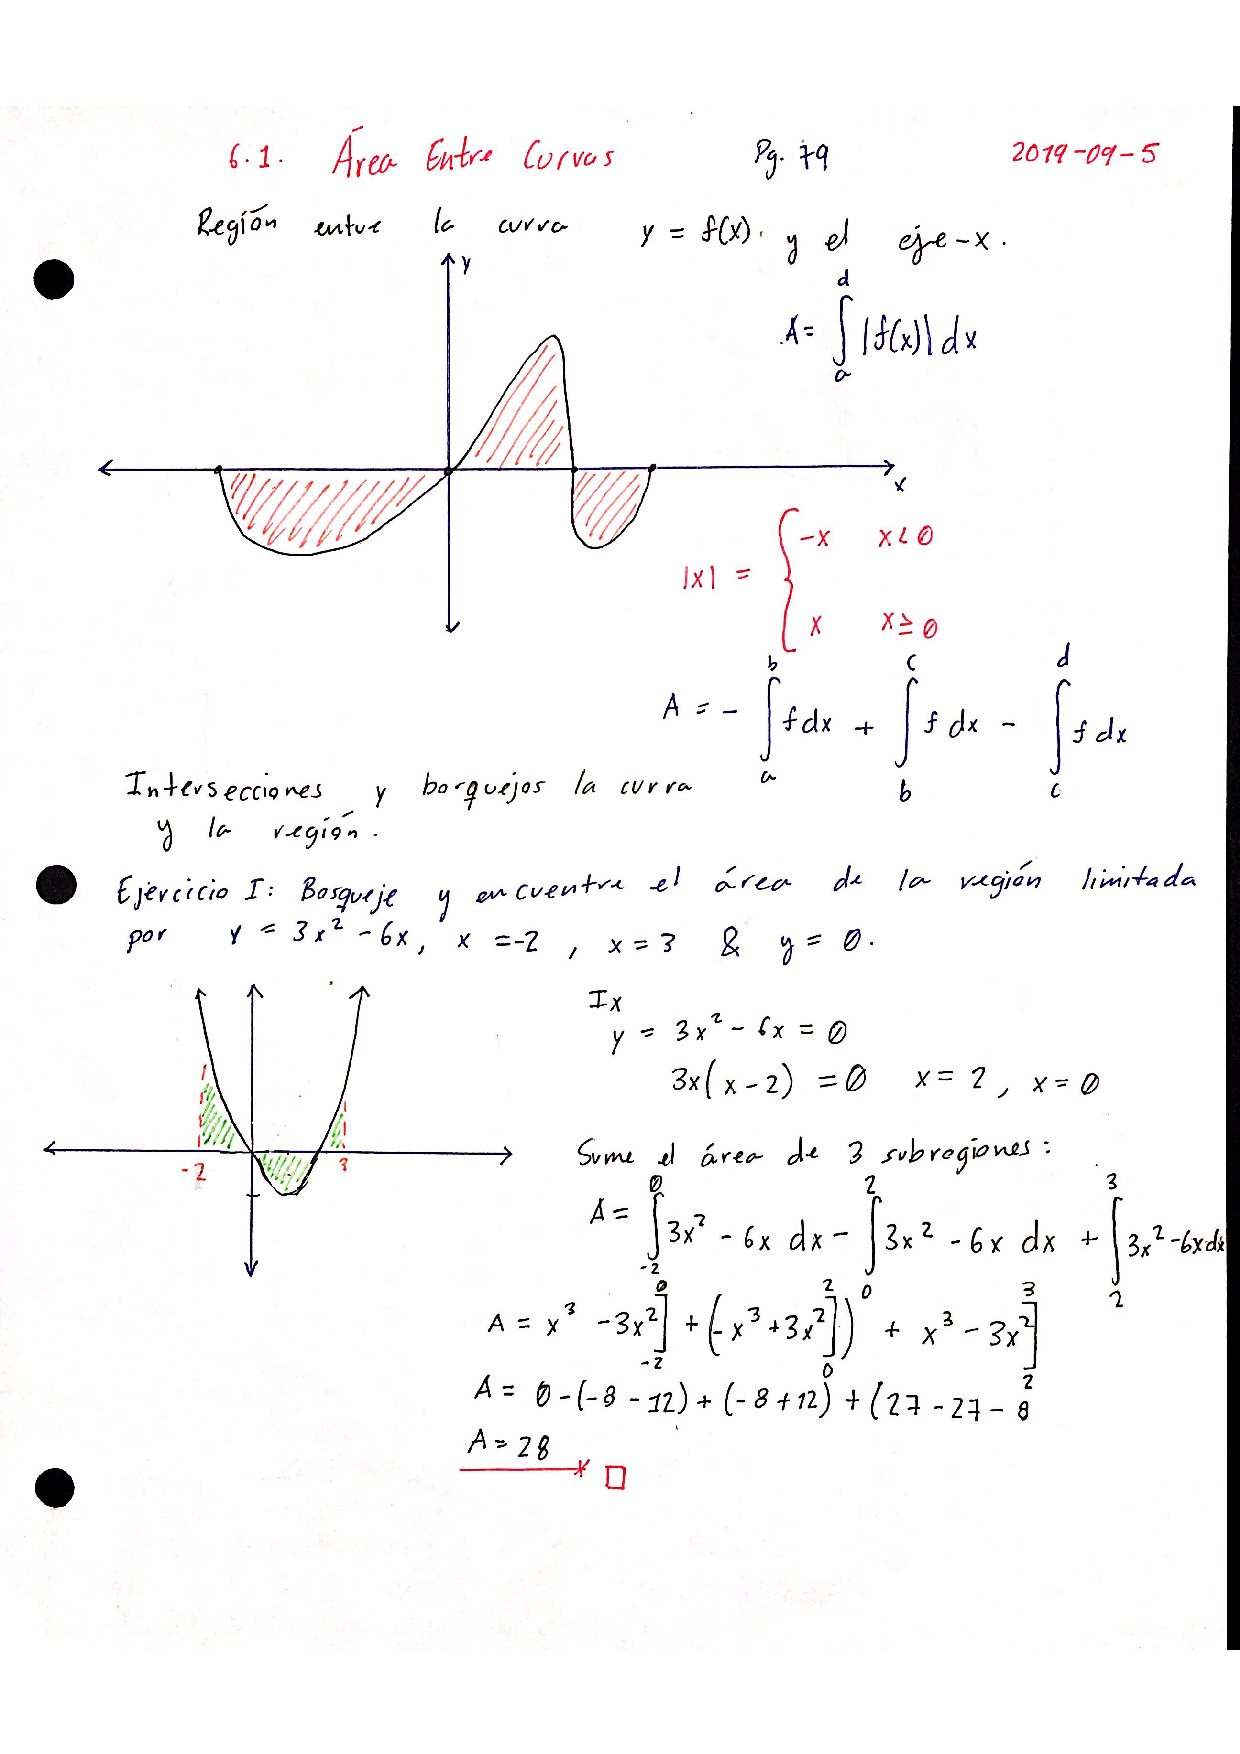
\includepdf[pages=-,pagecommand={\thispagestyle{plain}}]{pdf/MC_13-2019-09-05.pdf}


\chapter{Aplicación de la integración, integración respecto a y para encontrar áreas entre curvas, integración respecto a x para encontrar áreas entre curvas, introducción a \textbf{volúmenes}}
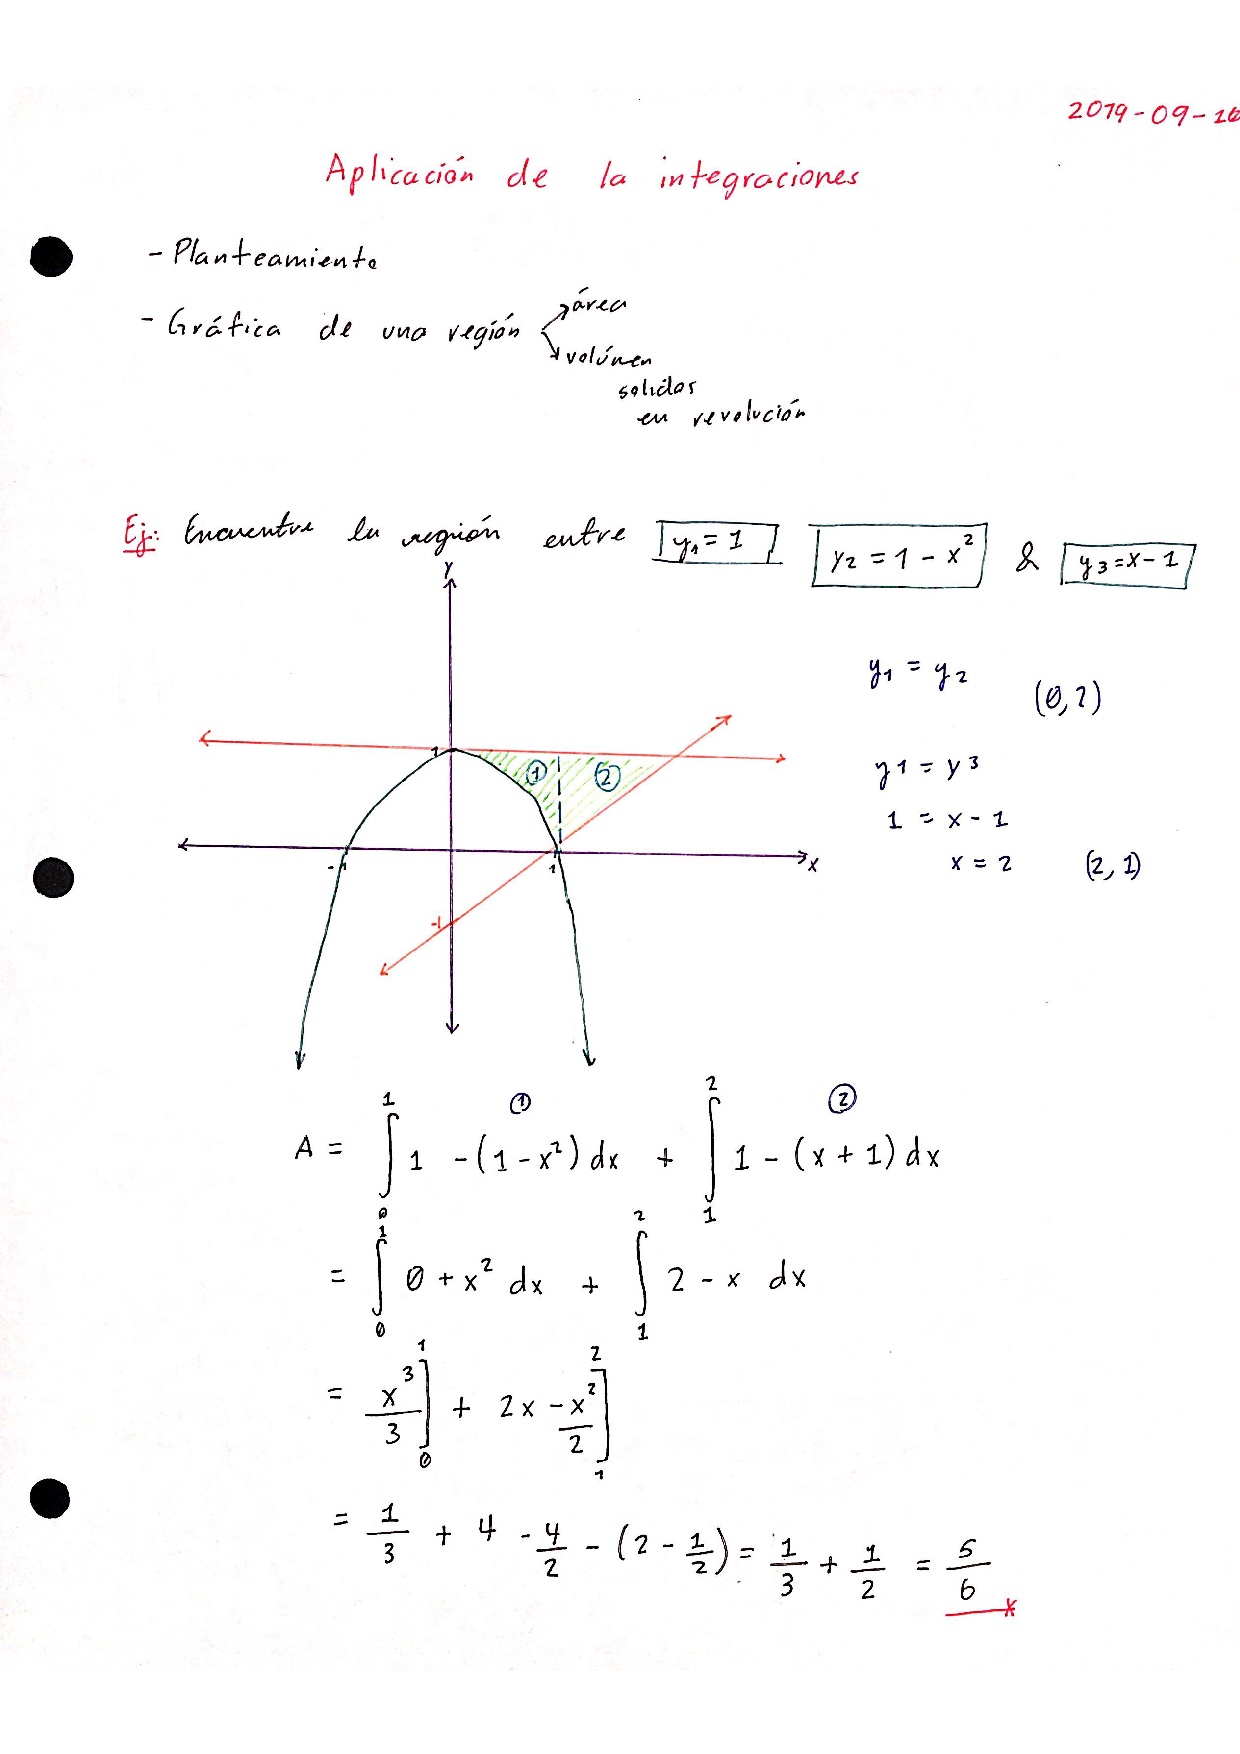
\includepdf[pages=-,pagecommand={\thispagestyle{plain}}]{pdf/MC_14-2019-09-10.pdf}


\chapter{Volúmenes, sólidos en revolución, cilíndros \& solidos huecos}
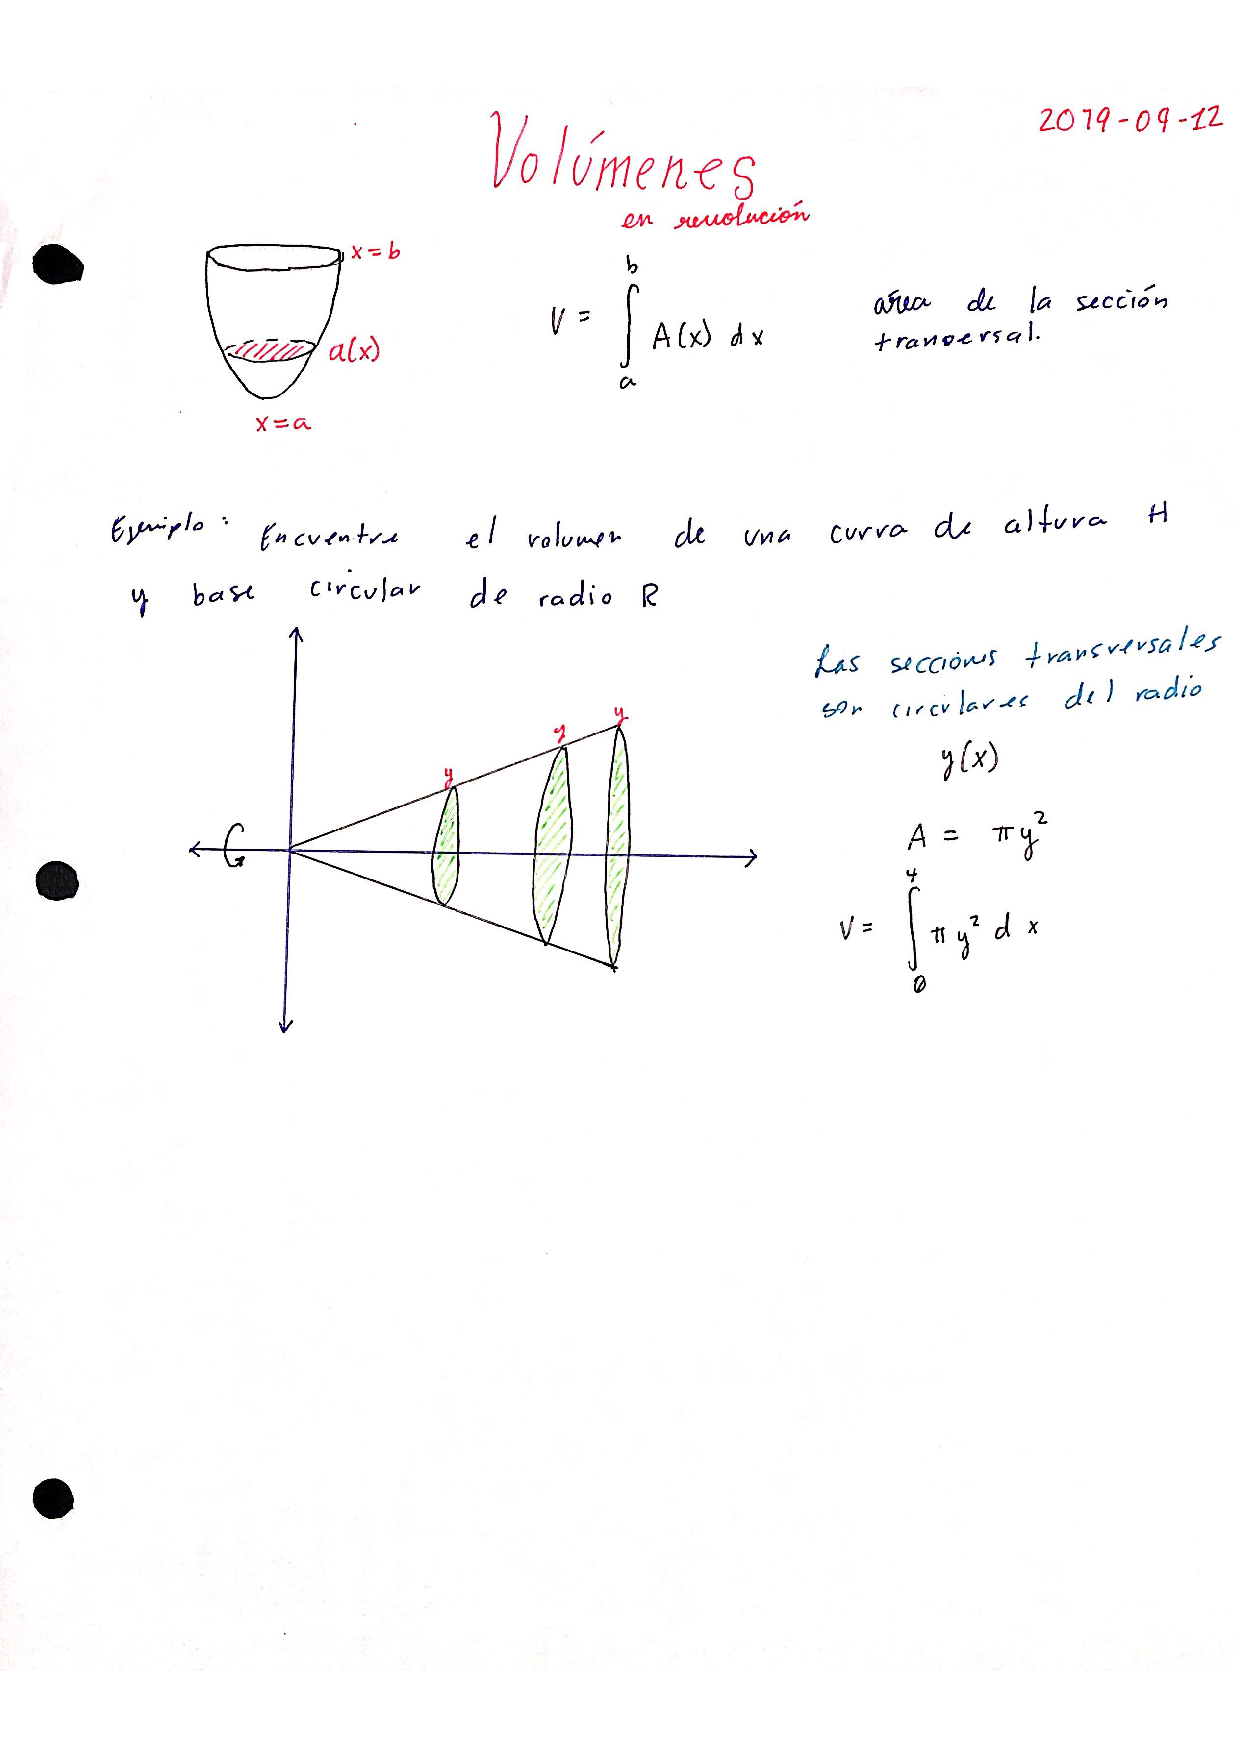
\includepdf[pages=-,pagecommand={\thispagestyle{plain}}]{pdf/MC_15-2019-09-12.pdf}

\chapter{Continuación de volúmenes, volúmenes con un cascarón cilíndrico.}
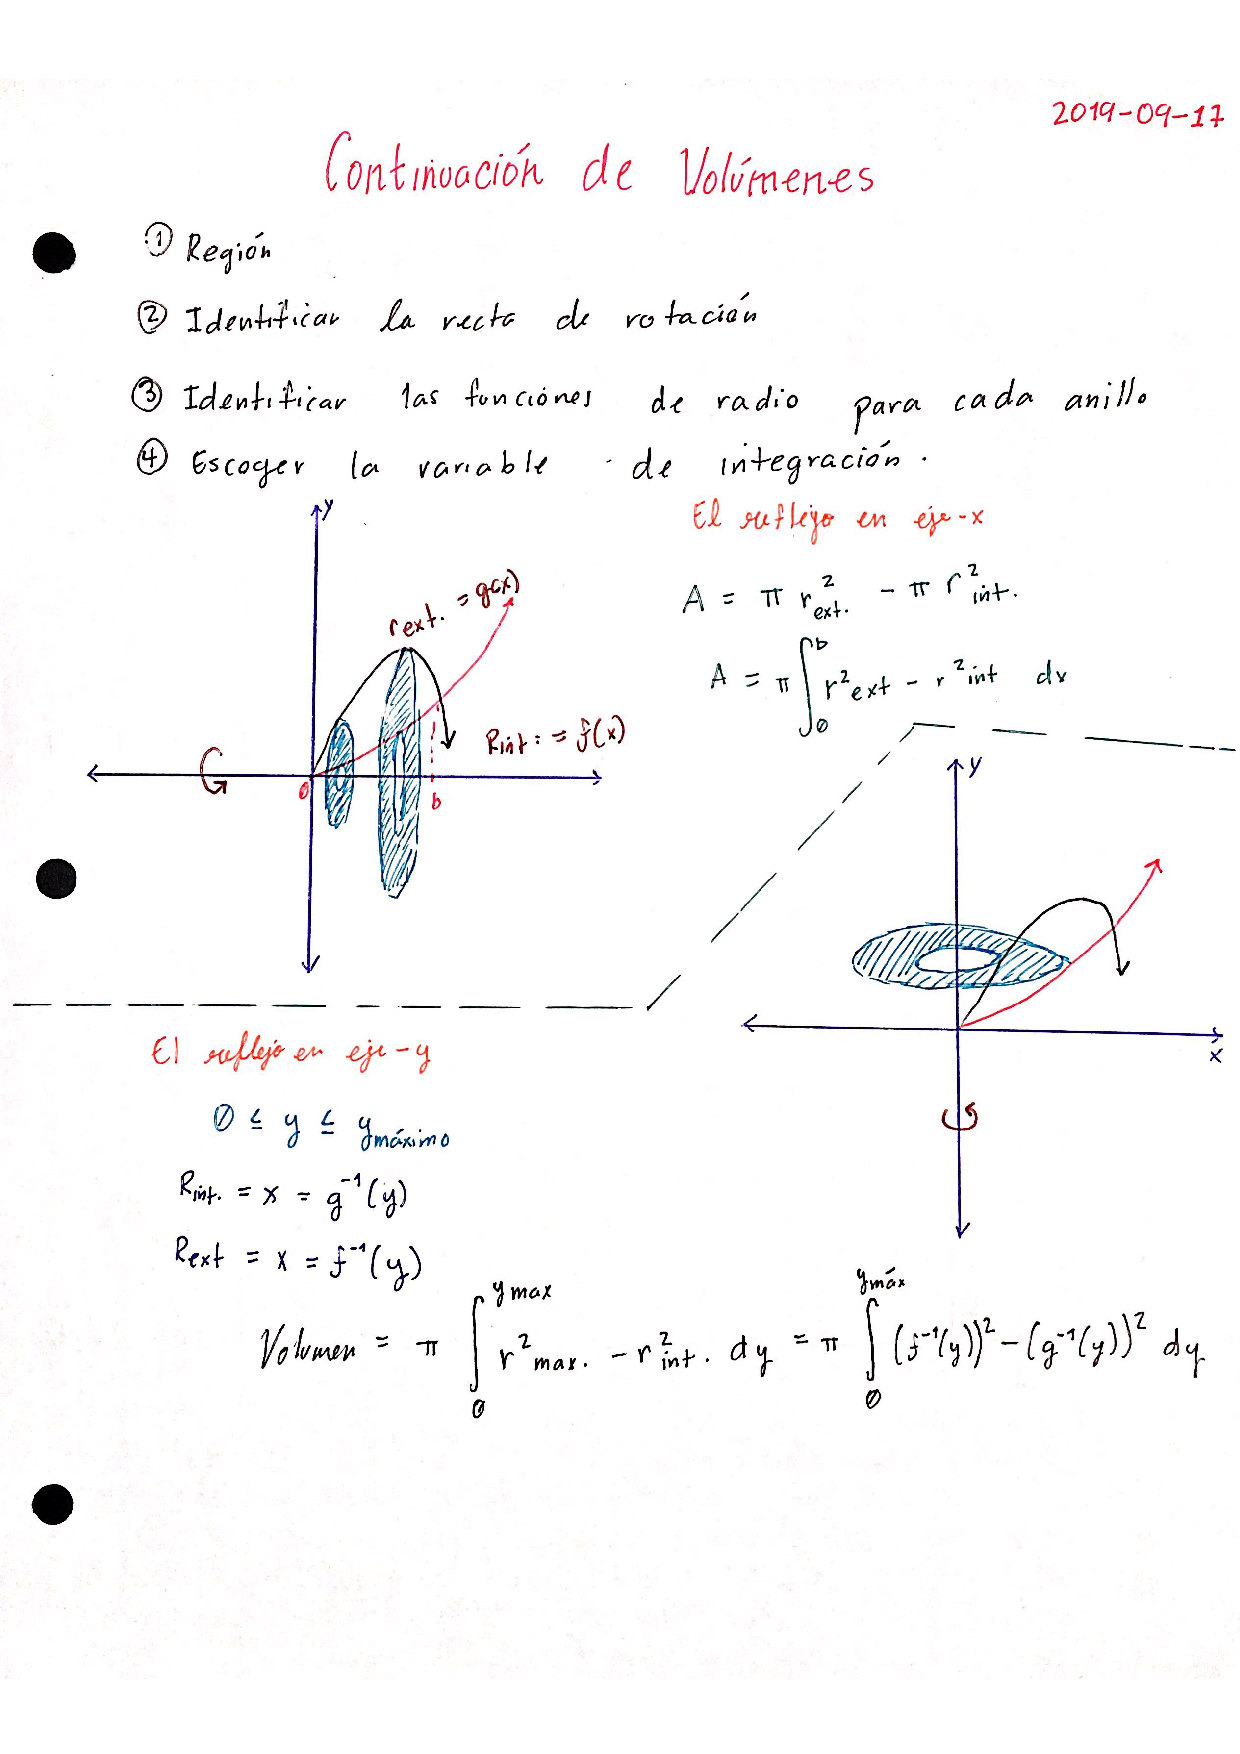
\includepdf[pages=-,pagecommand={\thispagestyle{plain}}]{pdf/MC_16-2019-09-17.pdf}


\chapter{Valor promedio de una función}
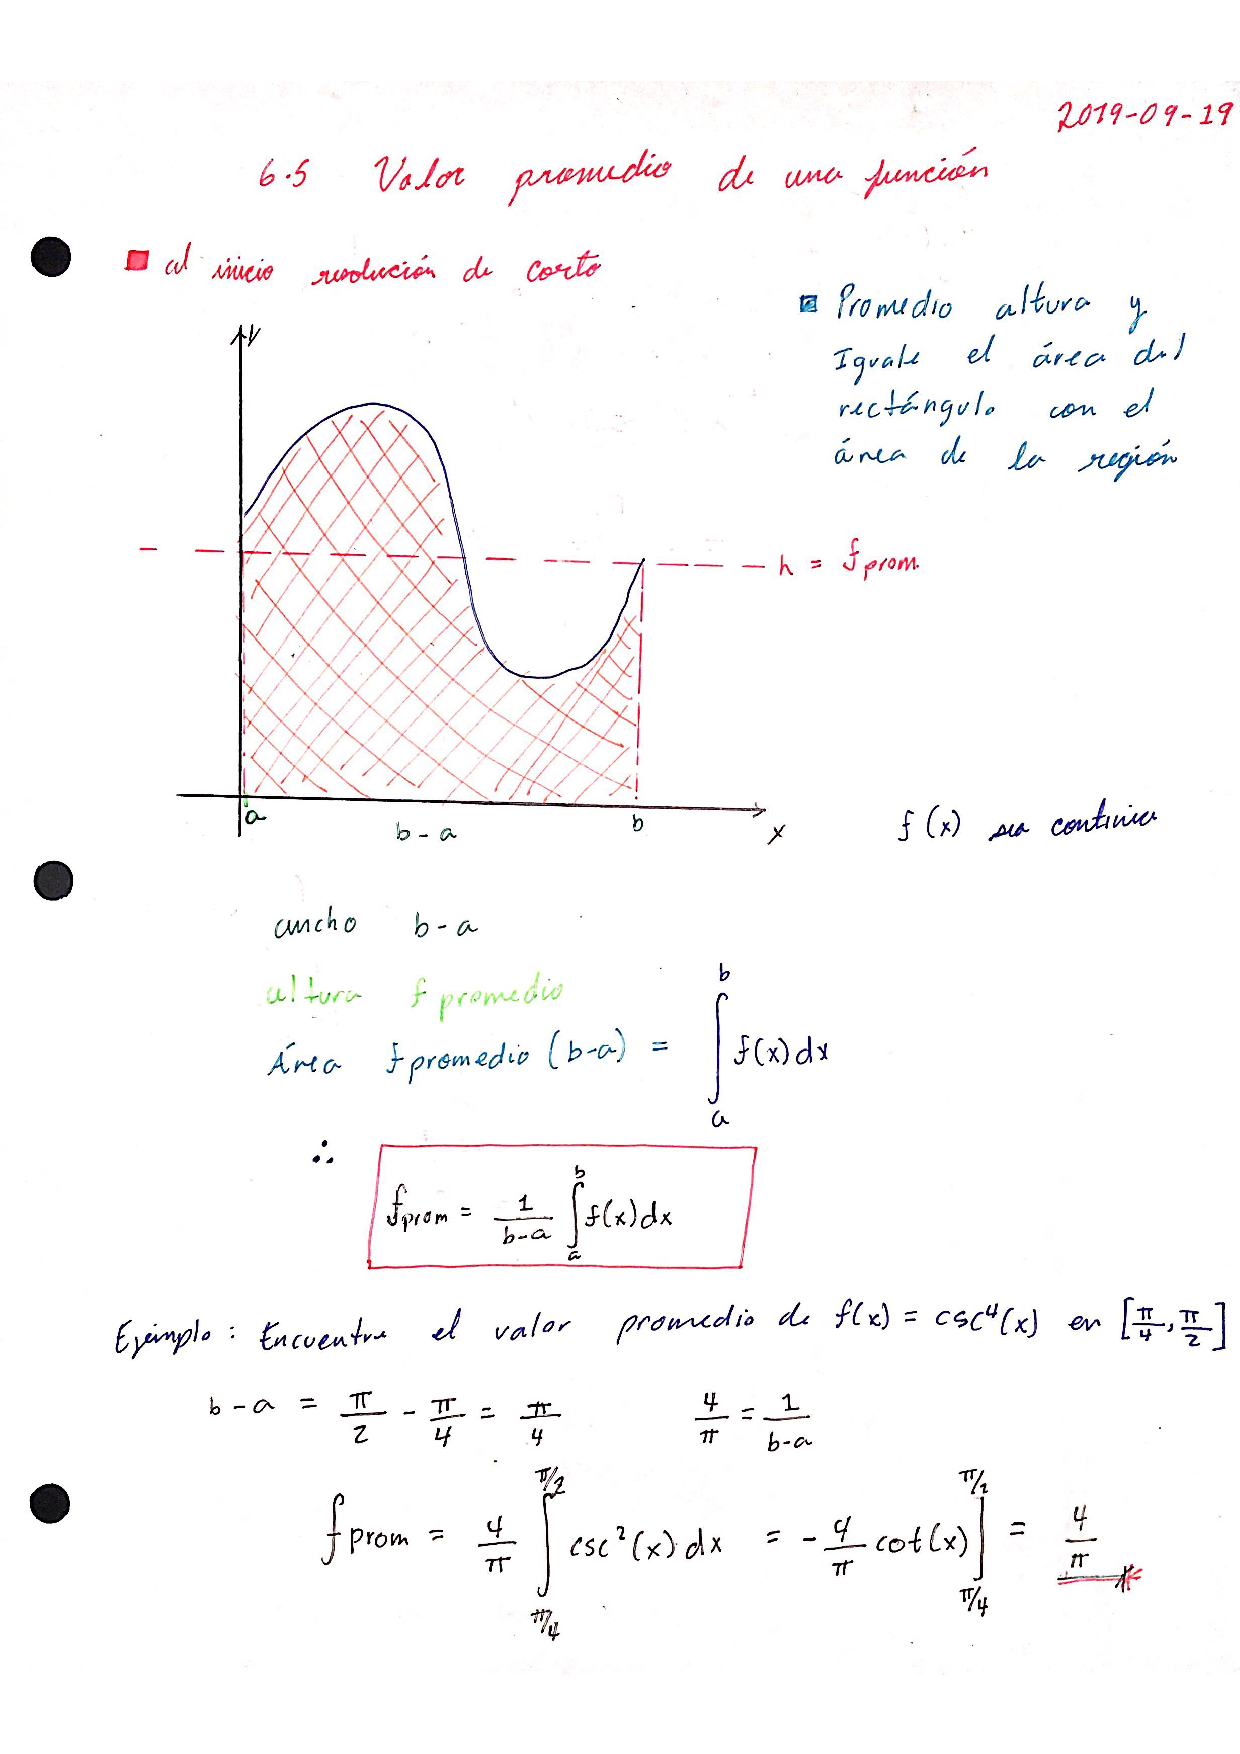
\includepdf[pages=-,pagecommand={\thispagestyle{plain}}]{pdf/MC_17-2019-09-19.pdf}

\chapter{Longitud de arco}
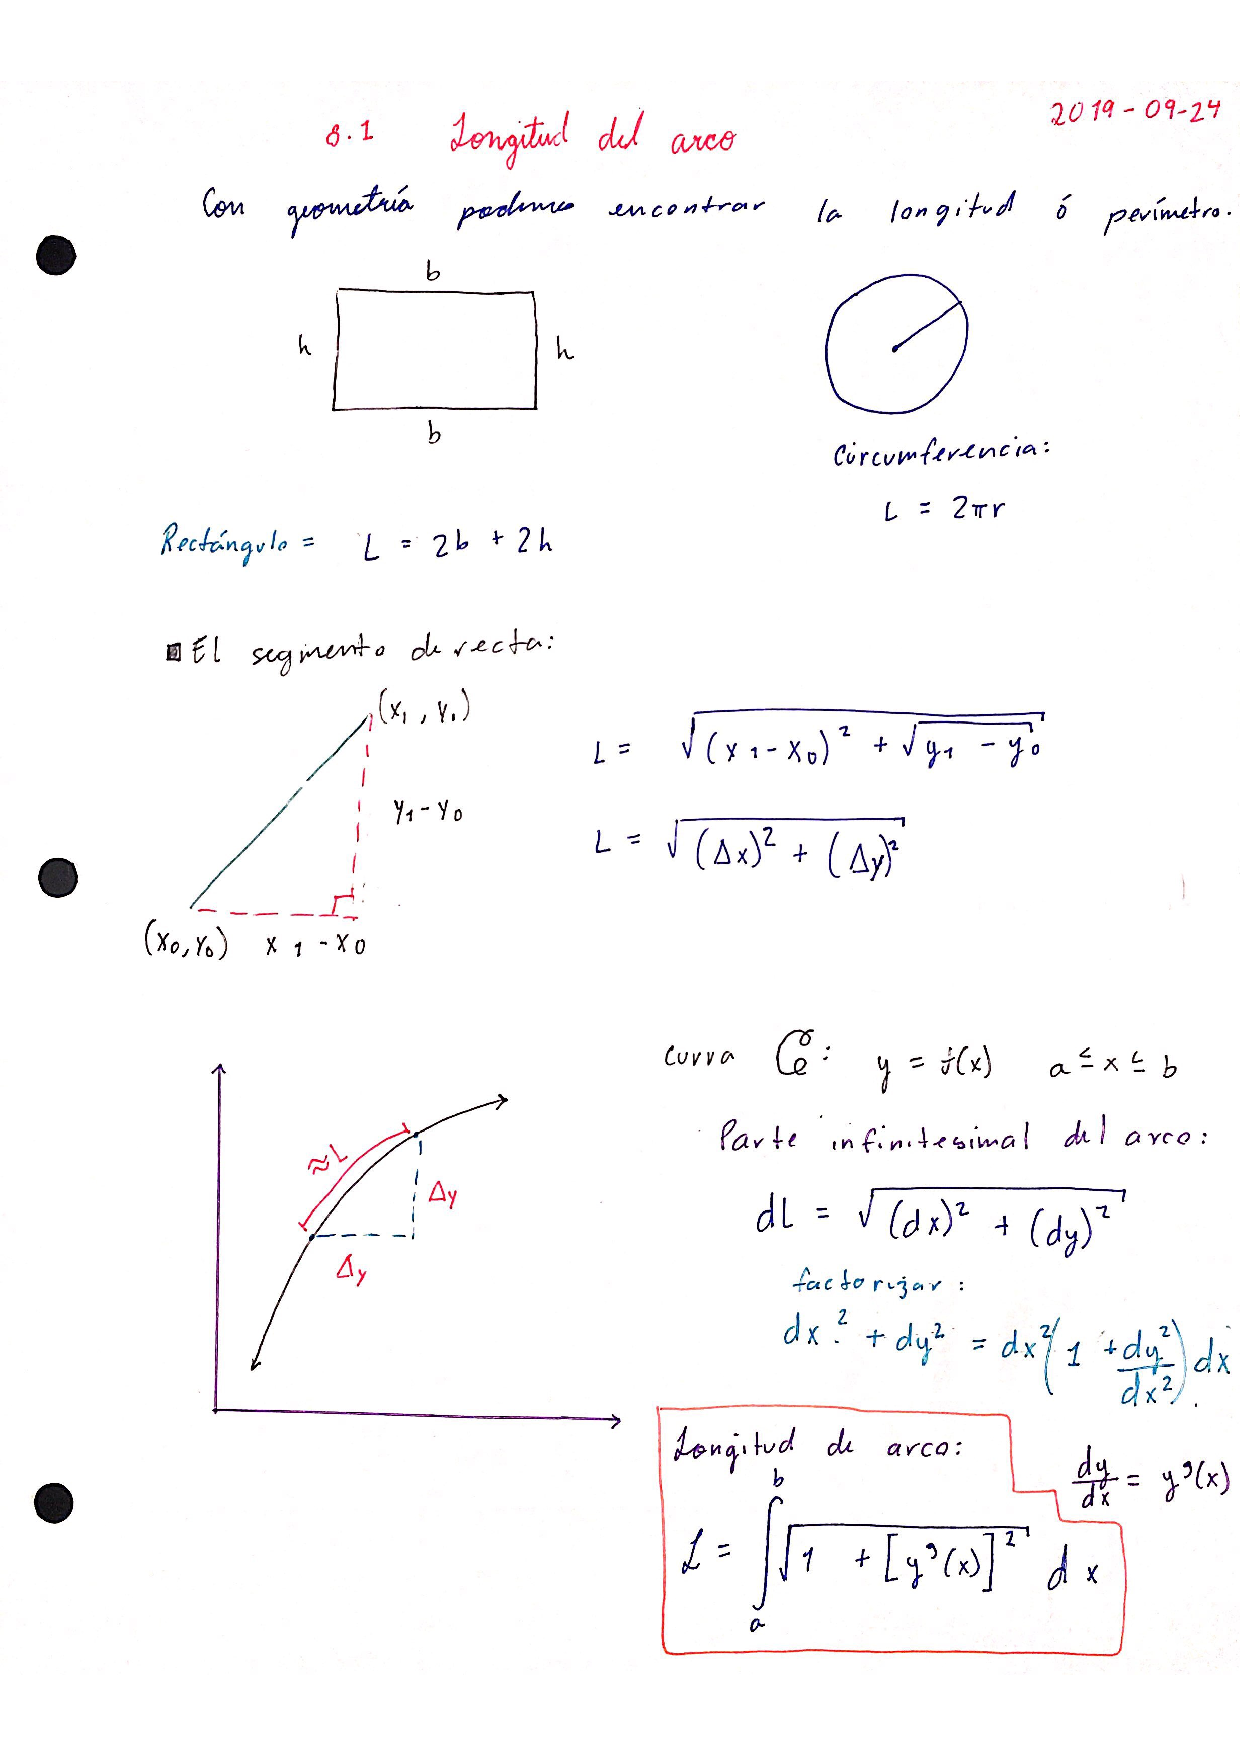
\includepdf[pages=-,pagecommand={\thispagestyle{plain}}]{pdf/MC_18-2019-09-24.pdf}

\chapter{Probabilidades, función de densidad, distribuciones de probabilidad comunes(tipo uniforme, tipo normal, tipo exponencial)}
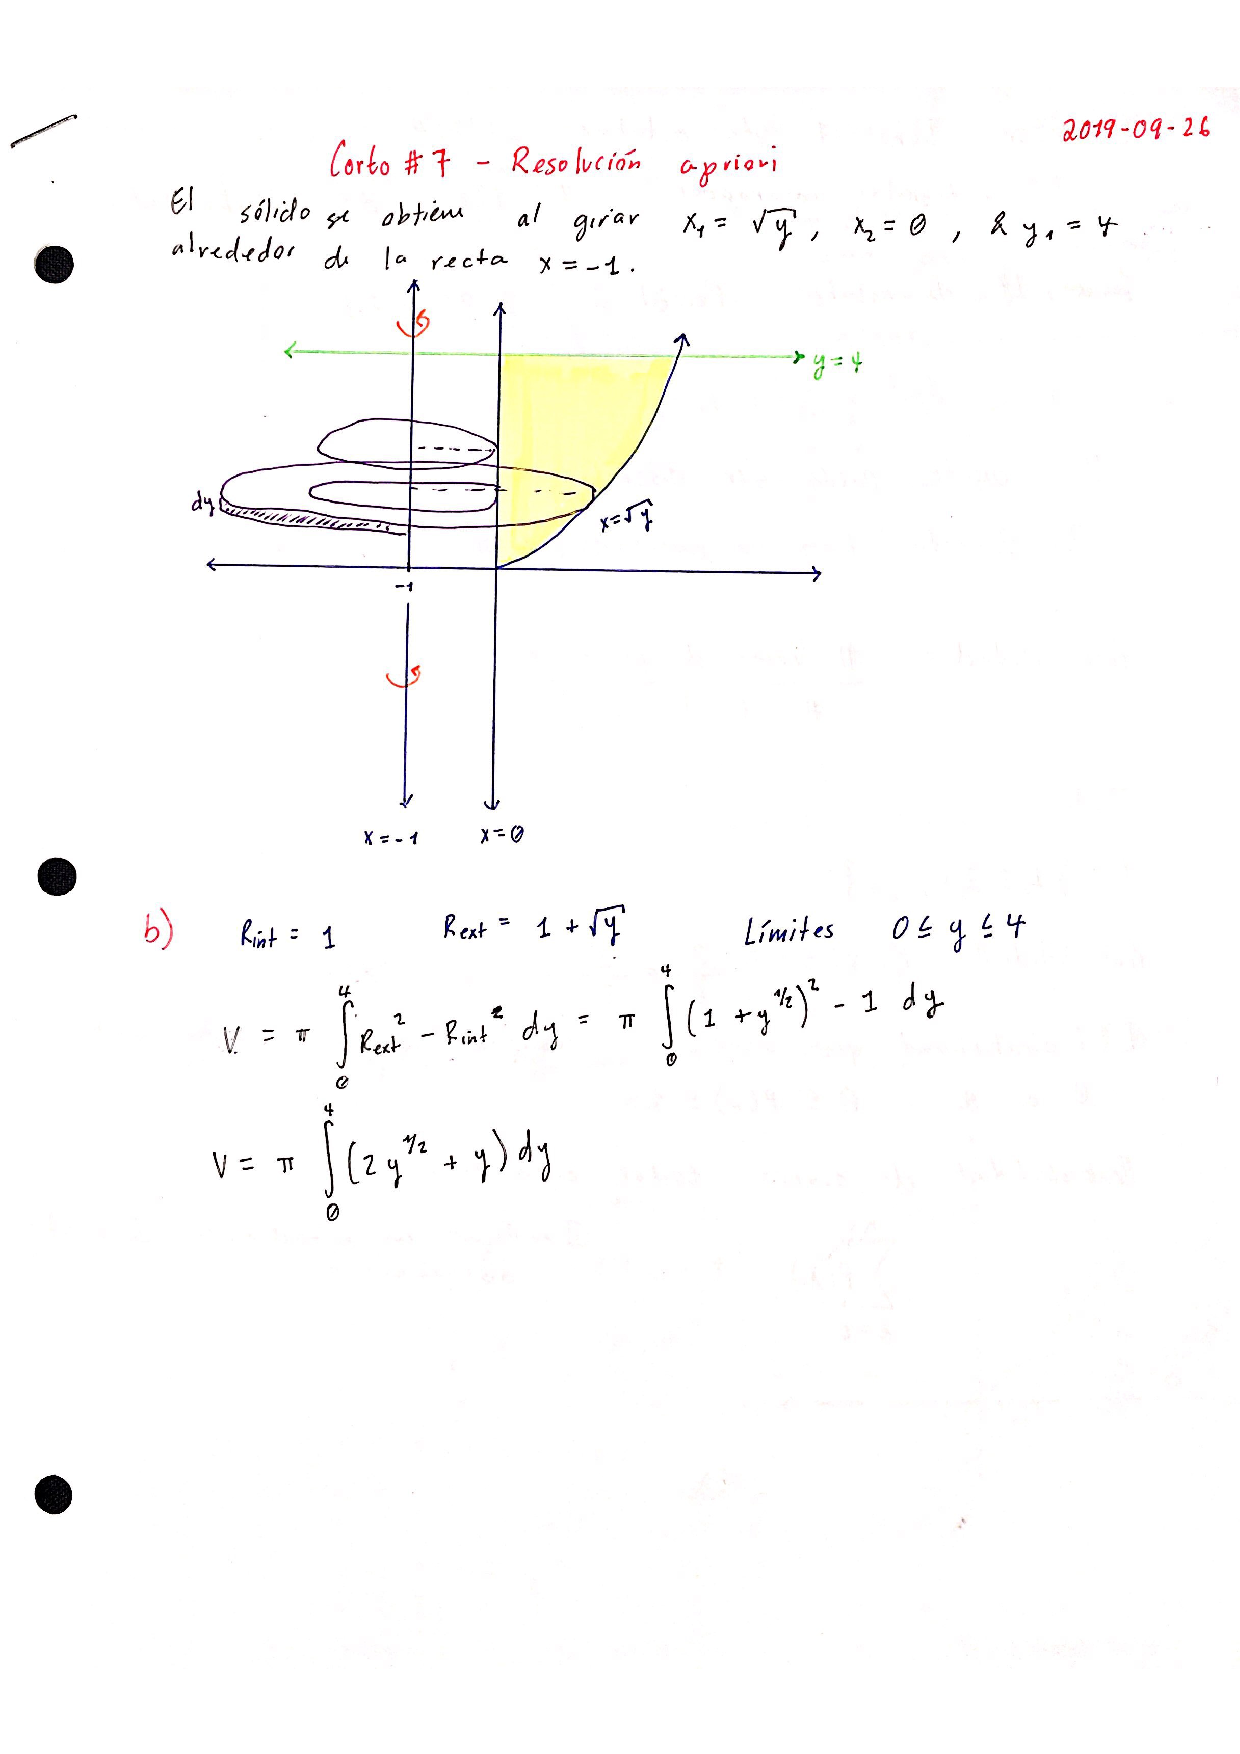
\includepdf[pages=-,pagecommand={\thispagestyle{plain}}]{pdf/MC_20-2019-09-26.pdf}

\chapter{Continuación Probabilidad}
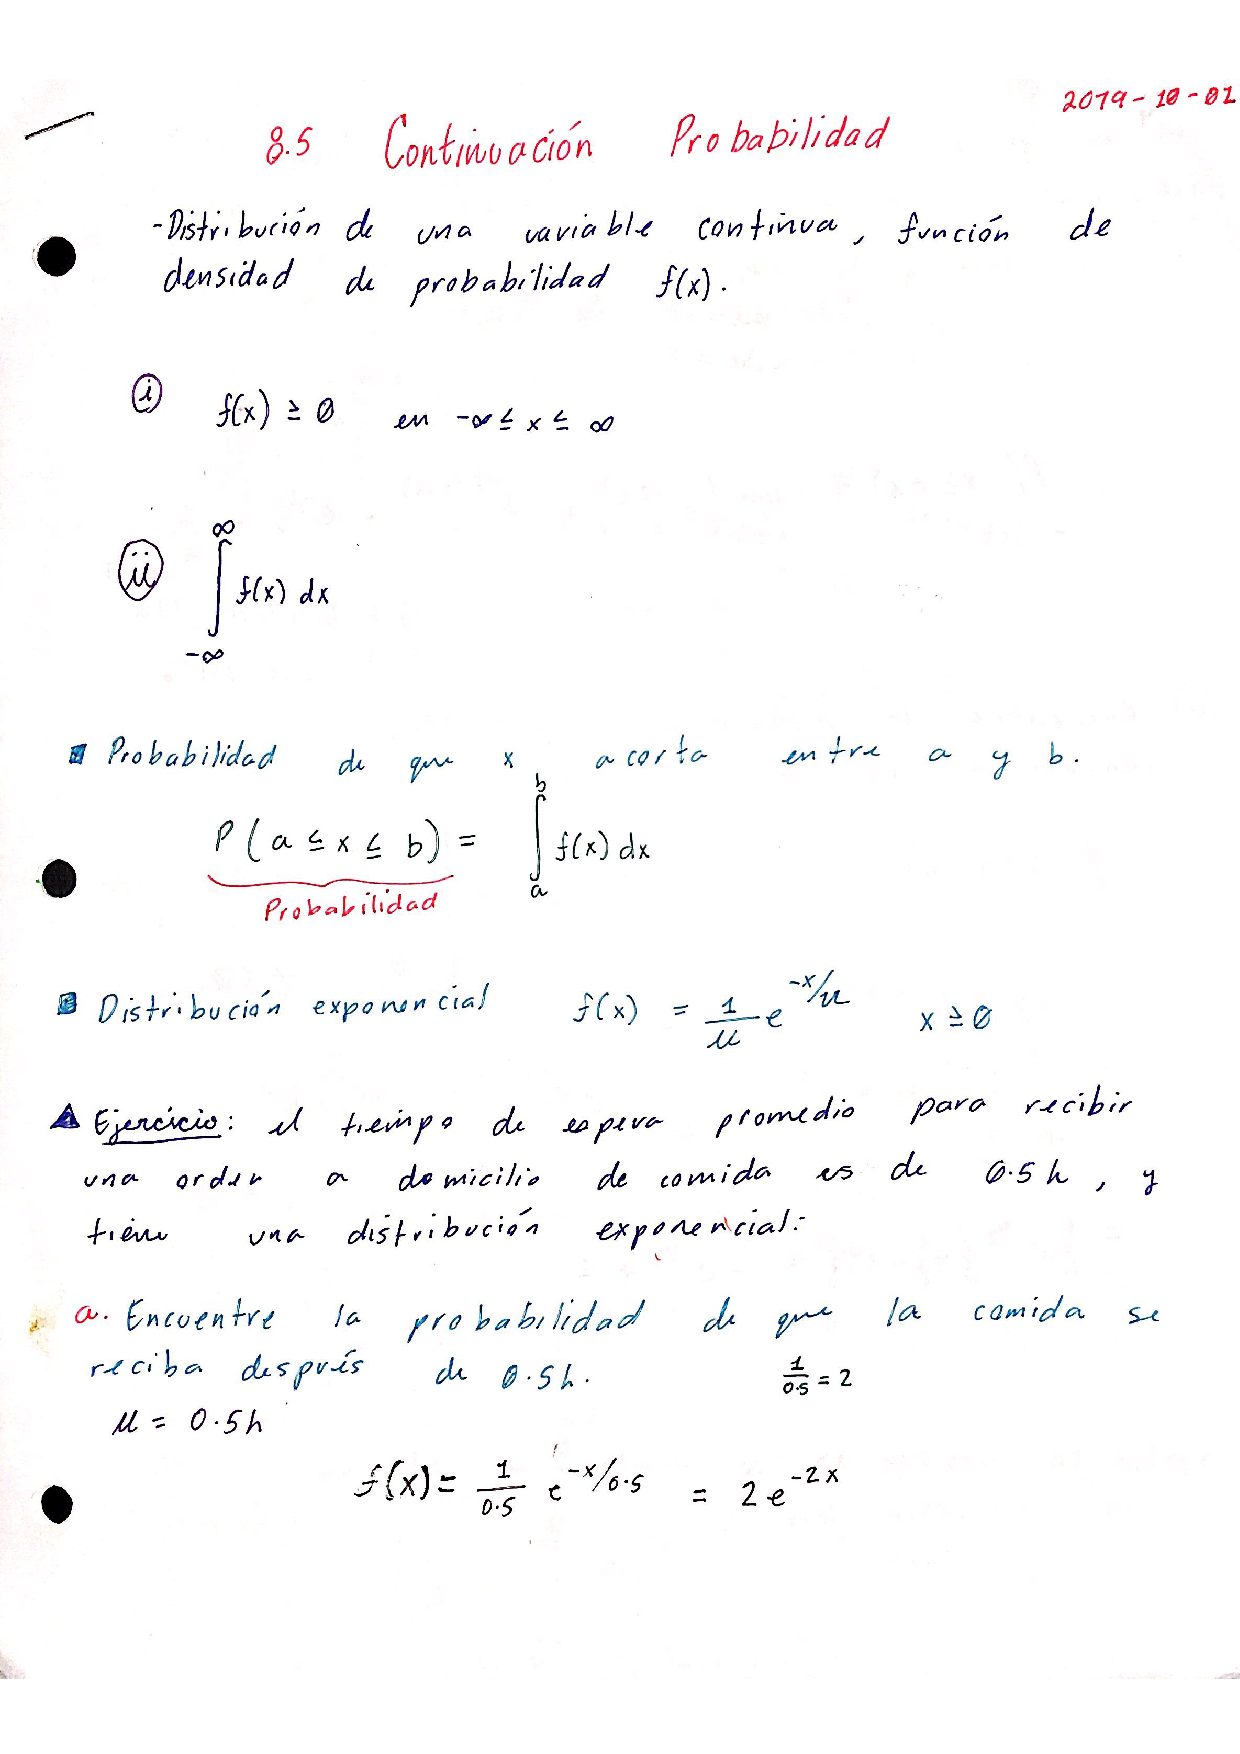
\includepdf[pages=-,pagecommand={\thispagestyle{plain}}]{pdf/MC_21-2019-10-01.pdf}

\chapter{Fracciones parciales \\ Caso 1: Factores lineales distintos \\ Caso 2: Factores lineales repetidos}
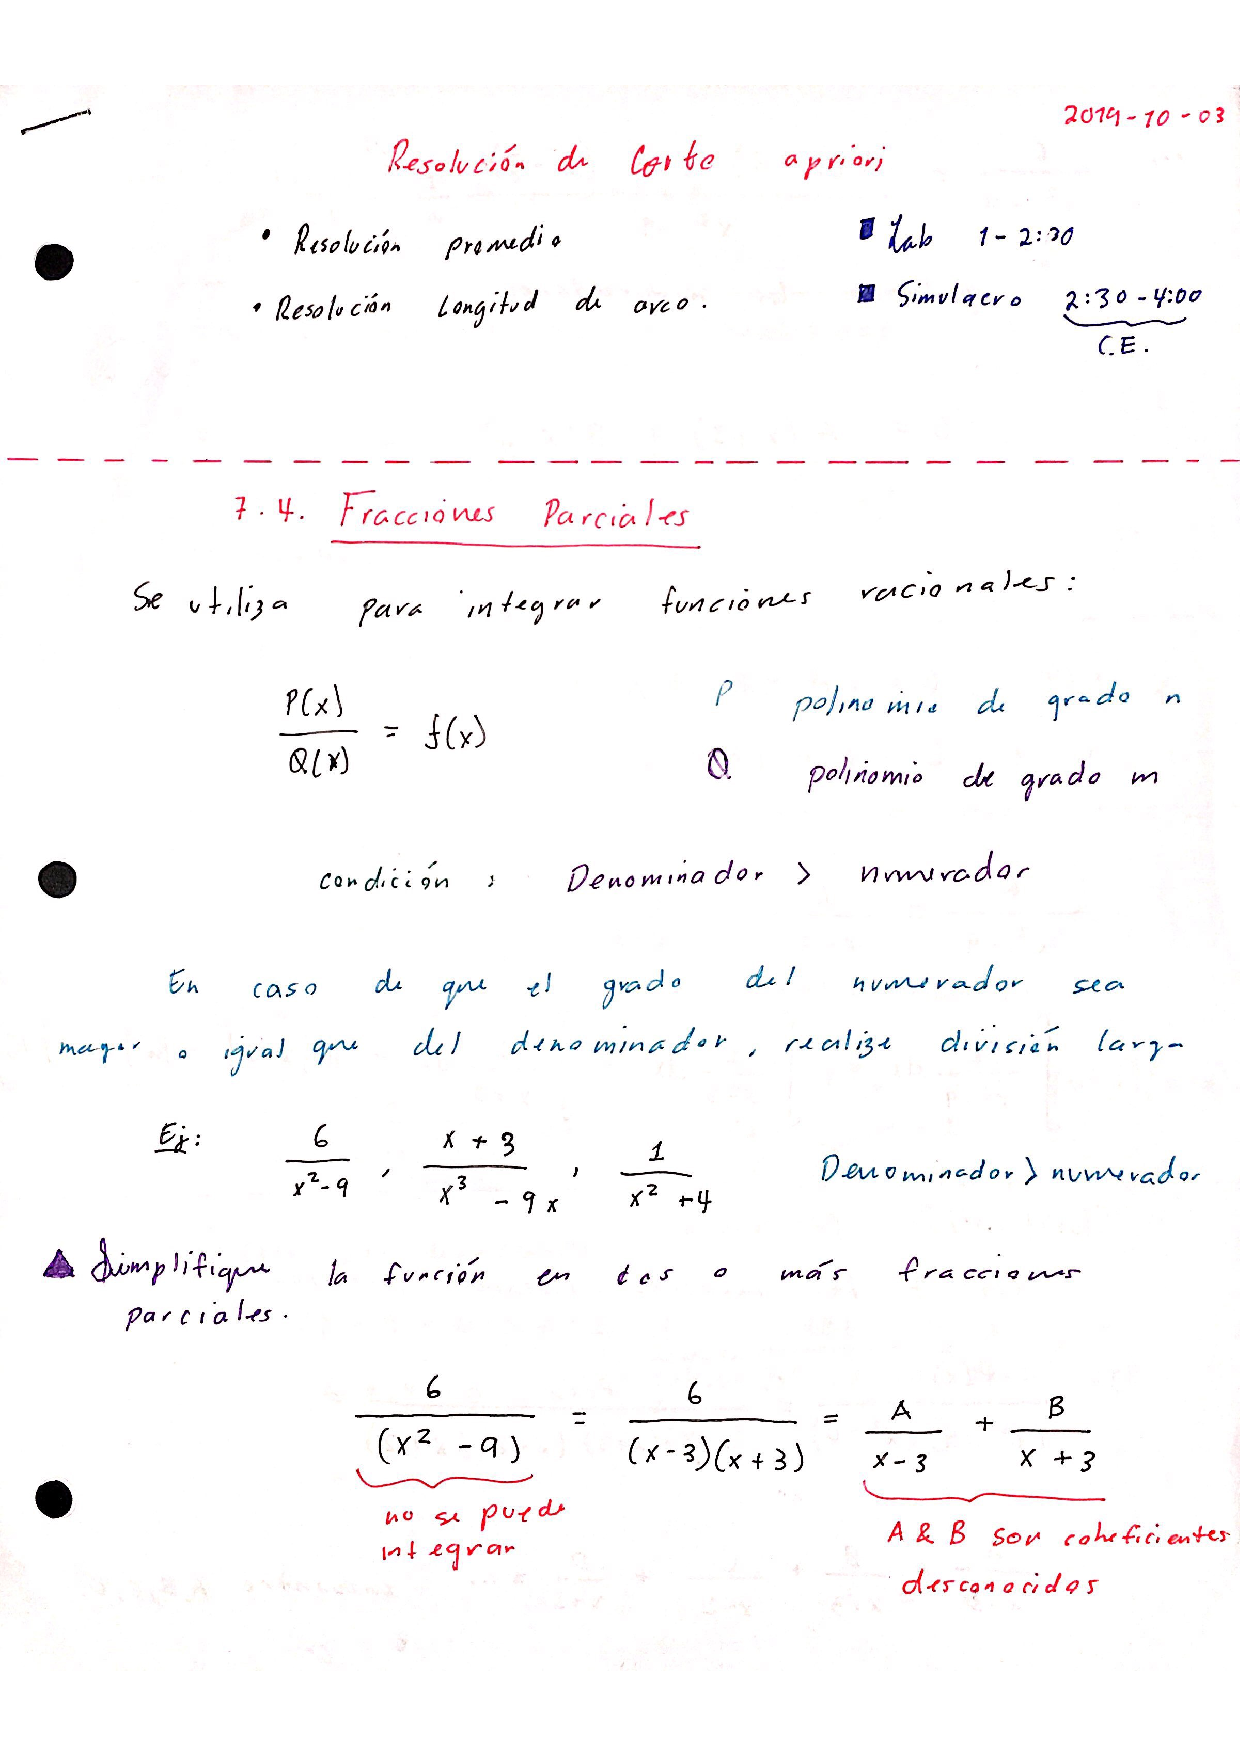
\includepdf[pages=-,pagecommand={\thispagestyle{plain}}]{pdf/MC_22-2019-10-03.pdf}

\chapter{Fracciones parciales \\ Caso 3: Factores cuadráticos irreducibles \\ Caso 4: Factores cuadráticos repetidos }
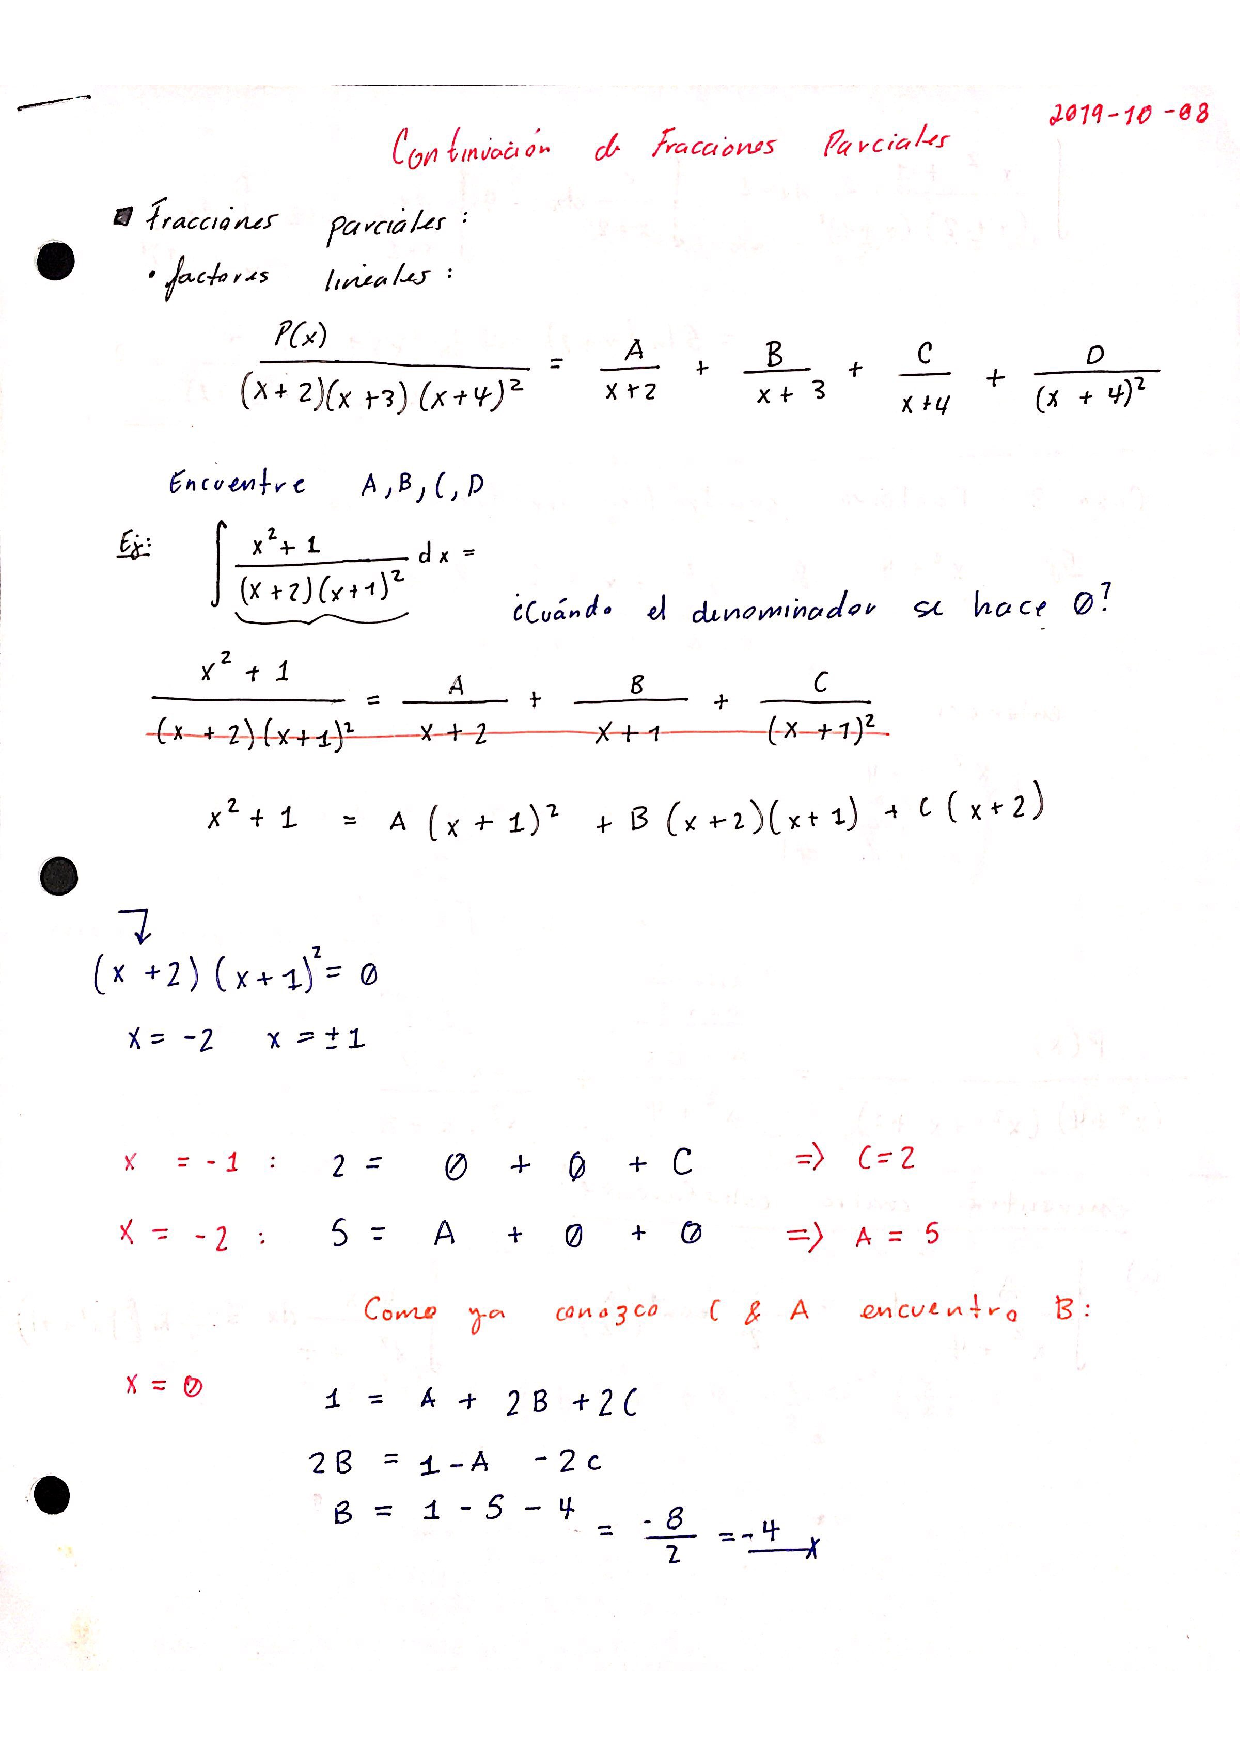
\includepdf[pages=-,pagecommand={\thispagestyle{plain}}]{pdf/MC_23-2019-10-08.pdf}





%%%%%%%%%%%%%%%%%%%%%%%%%%%%%%%%%%%%%%%%%%%%%%%%%%%%%%%%%%%%%%%%%%%%%%%%%%%%%%%%%%%%%%%%%%%%%%%%






\end{document}
